% Chapter: Rational Conjugacy: Pochhammer Priors and Gamma Ratios
% Macros
\DeclareRobustCommand{\rcPH}{\mathrm{PH}}
\DeclareRobustCommand{\rcPPH}{\mathrm{PPH}}
\DeclareRobustCommand{\rcTPH}{\mathrm{TPH}}
\DeclareRobustCommand{\rcGa}{\mathrm{Ga}}
\DeclareRobustCommand{\rcBe}{\mathrm{Be}}
\DeclareRobustCommand{\rcExp}{\mathrm{Exp}}
\DeclareRobustCommand{\rcNB}{\mathrm{NB}}
\DeclareRobustCommand{\rcPG}{\mathrm{PG}}
\DeclareRobustCommand{\rcCRT}{\mathrm{CRT}}
\DeclareRobustCommand{\rcPoi}{\mathrm{Poi}}
\DeclareRobustCommand{\rcR}{\mathcal{R}}
\DeclareRobustCommand{\rcP}{\mathcal{P}}
\DeclareRobustCommand{\rcM}{\mathcal{M}}
\DeclareRobustCommand{\rcK}{\mathcal{K}}
\DeclareRobustCommand{\rcone}{\mathbf{1}}
\DeclareRobustCommand{\rcgE}{\gamma_{\mathrm{E}}}

\chapter{Rational Conjugacy: Pochhammer Priors and Gamma Ratios}\label{ch:rc}
\chaptermark{Rational Conjugacy}
% Narrow 4.5in measure: allow extra interword stretch before reporting overfull lines.
\emergencystretch=3em

\begin{chaptersummary}
Pochhammer priors, introduced by \citet{rc:wang2024}, give conjugate Bayesian inference for concentration parameters that enter a likelihood through ratios of Gamma functions with integer shifts. This chapter develops the general theory of that family around a single principle, rational conjugacy: the Pochhammer family is not closed under Bayesian updating, but the proper rational densities on $\mathbb{R}^+$ are, and on that class every normalizing constant, moment and predictive probability is a finite sum of residues.

Five results follow, each generalizing or correcting a statement of \citet{rc:wang2024}. A general residue formula admits poles of arbitrary multiplicity anywhere in the cut plane, as required for Pitman Yor, where poles repeat, and for Erlang's loss system, where they are complex. The Mellin transform of a Pochhammer density is obtained in closed form on its maximal strip, delivering fractional and negative moments, $\E\log\alpha$, the exact tail index $b-m-d-1$ (with a second, probabilistic proof in Corollary~\ref{rc:cor:shape}), and a corrected reading of the Kullback Leibler risk bound: every $m$ attains the superefficient rate $N^{-1}\log N$, and $m=0$ merely minimizes the constant. A completely monotone representation then identifies $m=d=0$ on structural grounds: the half horseshoe is a scale mixture of exponentials whose mixing law is a size debiased sum of independent exponentials, so a latent scale reduces the prior to a tilt exactly as an inverse Gamma scale reduces the half Cauchy to a Gaussian. The consequence is practical. Wherever a Gamma prior on a concentration parameter admits an exact draw, the half horseshoe does too, at the cost of $b$ extra exponential variates; for Negative Binomial regression this yields a Gibbs sampler in which every block is a standard draw, no Metropolis step appears, and no residue is ever evaluated. An exponentially tilted family completes the picture, its normalizer a finite sum of exponential integrals, and the tilt removes the degree restriction $b\ge m+d+2$ altogether.

We then locate the boundary of the method: $\Gamma(\alpha+u)/\Gamma(\alpha+v)$ is rational if and only if $u-v\in\mathbb{Z}$, so Damsleth's \citeyearpar{rc:damsleth1975} conjugate class for the two parameter Gamma lies outside it, and we give three repairs, two of them exact, of which Poisson augmentation is the sharpest, together with a fourth that is not ours: the reciprocal Gamma mixtures of He, Polson and Xu reach the transcendental factor directly, and we set out the division of labour between augmentation and residues. A power law theorem shows the Negative Binomial, Beta, Pochhammer hierarchy generates $p(n)\sim Kn^{-(1+a)}(\log n)^{-\{2+\rcone(m\ge1)\}}$, so a Zipf exponent may be elicited as a prior hyperparameter. Applications include P\'olya urns, the Ewens sampling formula, Pitman Yor concentration, Yule processes and Erlang's formula, and a Negative Binomial regression study of two count data sets in which a $\rcGa(2,1)$ prior on the dispersion holds the posterior far below the near Poisson values the likelihood supports and doubles the width of the predictive bands, while the half horseshoe does not. Finally we quantify a limitation: the residue expansion is exact but ill conditioned, provably losing $n\log_{10}2$ digits in a solvable case, and we give three remedies.

Because this is a book about genetics, the running example is the concentration parameter $\theta$ of the Ewens sampling formula, the scaled mutation rate of the infinitely many alleles model, together with its Pitman Yor extension and the Hoppe urn that generates both. A dedicated section works the residue calculus by hand for a sample of four genes carrying two alleles, obtaining the normalizing constant, the posterior mean and the probability that the next gene carries a new allele as exact combinations of $\log2$ and $\log3$; shows how many digits double precision loses as the sample grows; gives an exact two line sampler for the half horseshoe; and analyses Corbet's Malayan butterflies, where a light tailed $\rcGa(2,1)$ prior of the kind used in the Dirichlet process literature moves the posterior for $\theta$ far below the maximum likelihood value while the half horseshoe leaves it in place.
\end{chaptersummary}

\section{Introduction}\label{rc:sec:intro}

Let $[x]^n=x(x+1)\cdots(x+n-1)=\Gamma(x+n)/\Gamma(x)$ be the rising factorial. A large part of applied probability depends on a concentration parameter $\alpha>0$ only through such symbols. The Dirichlet Multinomial likelihood is $\prod_k[\alpha_k]^{n_k}/[A]^N$; the Negative Binomial is $\prod_i[\alpha]^{n_i}\pi^{K\alpha}$; the Ewens sampling formula \citep{rc:ewens1972} is $\alpha^k/[\alpha]^n$; the Pitman Yor law of the block count is $\prod_{i<k}(\theta+i\sigma)/[\theta+1]^{n-1}$; the P\'olya urn probability of $k$ white in $n$ draws is $[a]^k[\beta]^{n-k}/[a+\beta]^n$. In each case the parameter is hard to learn: the log likelihood is generally not concave, and the standard responses are empirical Bayes point estimates \citep{rc:minka2000}, auxiliary variables \citep{rc:escobar1995}, or Metropolis steps.

For the readers of this book the most important instance is the Ewens sampling formula. In the infinitely many alleles model a sample of $n$ genes falls into $K_n$ allelic classes, and the probability of the observed configuration depends on the scaled mutation rate $\theta=4N_e\mu$ only through $\theta^{K_n}/[\theta]^n$ (Chapter~\ref{ch:esf}). The same symbol governs the Hoppe urn \citep{rc:hoppe1984}, in which the $i$th gene sampled is a new allele with probability $\theta/(\theta+i-1)$; the Dirichlet process concentration in species sampling and clustering; and, with one extra parameter, the Pitman Yor model. Two facts make $\theta$ an awkward parameter. The information about it grows only like $\log n$ (Section~\ref{rc:sec:ewens}), so a sample of thousands of genes pins it down less well than a sample of a dozen pins down a normal mean; and its plausible range spans several orders of magnitude, from $\theta<1$ for a nearly monomorphic locus to $\theta$ in the hundreds for a hypervariable one. A prior for $\theta$ must therefore be heavy tailed, and a posterior for it must be computed with care. This chapter supplies both.

\citet{rc:wang2024}, hereafter WP, introduced the Pochhammer family
\begin{equation}\label{rc:eq:ph}
p(\alpha\mid m,a,b,c)\;\propto\;\frac{[\alpha]^m}{[c\alpha+a]^b},\qquad \alpha\ge0,
\end{equation}
with $m,b$ nonnegative integers, $b\ge m+2$, $a,c>0$, and its size biased extension $\rcPPH(m,a,b,c,d)\propto\alpha^d[\alpha]^m/[c\alpha+a]^b$, of which \eqref{rc:eq:ph} is the case $d=0$.\footnote{Definition 2 of \citet{rc:wang2024} states the case as $d=1$; the intended convention is $d=0$, which we adopt throughout.} WP establish conjugacy for the Dirichlet Multinomial concentration parameter, closed form normalizers by residues when all poles are simple, and that the choice $m=0$, $b=2$ behaves like a horseshoe on the half line. Everything below takes that paper as its starting point.

Five questions are left open by that treatment. Which likelihoods does the family serve, and is it the right family? What happens at repeated and complex poles? How far does the calculus reach towards the Gamma shape parameter, and towards Damsleth's \citeyearpar{rc:damsleth1975} conjugate class in particular? What count distribution does the hierarchy induce? And is the closed form usable in practice? The organizing idea fits in a sentence.

\begin{quote}
\emph{Rational conjugacy.} Proper rational densities on $\mathbb{R}^+$ are conjugate to rational likelihoods, because rational functions form a field; partial fractions then reduce every integral to elementary residues.
\end{quote}

Pochhammer symbols are tractable only because integer shifts make them polynomials, a remark that sounds trivial and is not: Proposition~\ref{rc:prop:boundary} turns it into an exact criterion for membership, and thereby into an exact description of where the method stops.

\subsection*{What is new}

Table~\ref{rc:tab:map} maps each result of \citet{rc:wang2024} to its generalization. Three statements in that paper are also sharpened or corrected: the moment formula extends from integer to complex order (Theorem~\ref{rc:thm:mellin}); the heavy tail proposition is replaced by the exact regular variation index (Corollary~\ref{rc:cor:tail}); and the claim that $m=0$ is required for Kullback Leibler superefficiency is corrected, since every $m$ attains the rate and $m=0$ only minimizes the constant (Corollary~\ref{rc:cor:rate}). The last correction removes the stated justification for the default prior, and Theorem~\ref{rc:thm:cm} supplies a better one in its place.

\begin{table}[htbp]
\centering\small
\begin{tabular}{@{}>{\raggedright\arraybackslash}p{1.75in}>{\raggedright\arraybackslash}p{2.6in}@{}}
\toprule
\citet{rc:wang2024} & This chapter\\
\midrule
Residues, simple poles only; one double root example; general recipe deferred & Theorem~\ref{rc:thm:residue}: arbitrary multiplicity, arbitrary complex location, improper case included\\
Integer moments by size biasing, $b\ge m+d+2$ & Theorem~\ref{rc:thm:mellin}: Mellin transform on the maximal strip; fractional, negative and log moments\\
Their Proposition 1: tail is heavier than exponential & Corollary~\ref{rc:cor:tail}: regularly varying with exact index $b-m-d-1$\\
Their Proposition 2: prior mass $\asymp\varepsilon^{1/2}$, ``$m=0$ needed'' & Corollary~\ref{rc:cor:rate}: rate $N^{-1}\log N$ for all $m$, constant $\{1+\rcone(m\ge1)\}/2$\\
Conjugacy for DM, NB, NM, GDM, Yule Simon, Ewens & Definition~\ref{rc:def:class} and Proposition~\ref{rc:prop:conj}: characterization and minimality of the rational class\\
NB with coupled Beta prior, their Figure 3 sparsity patterns & Theorem~\ref{rc:thm:zipf}: exact power law tail $Kn^{-(1+a)}(\log n)^{-\{2+\rcone(m\ge1)\}}$\\
``Default horseshoe type prior'' with $m=0$, $b=2$ & Theorem~\ref{rc:thm:cm}: $m=d=0$ is exactly the completely monotone case; scale mixture of exponentials\\
Metropolis within Gibbs for heterogeneous $\alpha$ & Algorithms 1 and 2: tilted family, and a sampler with every block exact and no residues\\
Residue conditioning not discussed & Proposition~\ref{rc:prop:cond}: exponential ill conditioning, proved in a solvable case, and three remedies\\
``Further calibration required beyond DM'' & Sections~\ref{rc:sec:gamma} to \ref{rc:sec:genetics}: Gamma shapes, urns, Ewens and Pitman Yor, Yule, credibility, Erlang\\
\bottomrule
\end{tabular}
\caption{Correspondence between the earlier results and their generalizations here.}\label{rc:tab:map}
\end{table}

\section{Rational Conjugacy}\label{rc:sec:rational}

\subsection{The class}

\begin{definition}[Pochhammer rational likelihood]\label{rc:def:class}
A likelihood $L$ belongs to $\rcR$ if
\begin{equation}\label{rc:eq:classR}
L(\alpha)\;=\;\kappa\,\frac{\prod_{j=1}^{J}[u_j\alpha+v_j]^{p_j}}{\prod_{l=1}^{J'}[w_l\alpha+x_l]^{q_l}},\qquad u_j\ge0,\ v_j\ge0,\ w_l>0,\ x_l>0,
\end{equation}
with $\kappa$ free of $\alpha$ and $p_j,q_l$ nonnegative integers. Let $\rcP$ denote the set of probability densities on $\mathbb{R}^+$ that are rational functions with no poles in $[0,\infty)$.
\end{definition}

Every $L\in\rcR$ is rational with all poles in the open left half plane, and $\rcR$ is closed under products, so independent experiments compound. The following is elementary but is the reason for everything that follows, and it says that $\rcP$ is not merely convenient but forced.

\begin{proposition}[Conjugacy and minimality]\label{rc:prop:conj}
(i) If $p\in\rcP$ and $L\in\rcR$ then $p(\cdot\mid\text{data})\propto Lp$ lies in $\rcP$, provided $\deg(\text{denominator})\ge\deg(\text{numerator})+2$ after cancellation. (ii) $\rcPH(m,a,b,c)\subset\rcPPH(m,a,b,c,d)\subset\rcP$. (iii) The Pochhammer family is itself \emph{not} closed. Updating $\rcPPH(m,a,b,c,d)$ by \eqref{rc:eq:classR} multiplies the numerator by $\prod_j[u_j\alpha+v_j]^{p_j}$ and adjoins poles at $-(x_l+i-1)/w_l$, $i=1,\dots,q_l$, so the posterior is again Pochhammer if and only if every $u_j\alpha+v_j$ and $w_l\alpha+x_l$ is an affine reparametrization of $\alpha$ and of $c\alpha+a$ respectively. Otherwise the pole set strictly grows. Since $w_l$ and $x_l$ range over all of $(0,\infty)^2$ and multiplicities compound, the closure of the Pochhammer family under $\rcR$ updating contains every element of $\rcP$ with real poles and real nonpositive numerator roots whose numerator and denominator retain the initial prior factors, and no smaller family of densities is closed.
\end{proposition}

\begin{table}[htbp]
\centering\small
\setlength{\tabcolsep}{4pt}
\begin{tabular}{@{}>{\raggedright\arraybackslash}p{1.45in}>{\raggedright\arraybackslash}p{1.75in}>{\raggedright\arraybackslash}p{1.05in}@{}}
\toprule
Model & $L(\alpha)$ up to constants & Section\\
\midrule
Dirichlet Multinomial & $\prod_k[\alpha]^{n_k}/[K\alpha]^N$ & \citet{rc:wang2024}\\
Heterogeneous DM, Gibbs conditional & $[\alpha_k]^{n_k}/[\alpha_k+A_{-k}]^N$ & \ref{rc:sec:globallocal}\\
Negative Binomial, $\pi$ integrated & $\prod_k[\alpha]^{n_k}[c\alpha+a]^b/\allowbreak[(c+K)\alpha+a]^{N+b}$ & \ref{rc:sec:nb}\\
Negative Multinomial & $\alpha/[\alpha+N]^{K+1}$ & \citet{rc:wang2024}\\
Beta Binomial, P\'olya urn & $\prod_i[\alpha]^{y_i}[\beta]^{n_i-y_i}/[\alpha+\beta]^{n_i}$ & \ref{rc:sec:urn}\\
Ewens, Dirichlet process & $\alpha^k/[\alpha]^n$ & \ref{rc:sec:ewens}\\
Pitman Yor, $\sigma$ fixed & $\prod_{i=1}^{k-1}(\theta+i\sigma)/[\theta+1]^{n-1}$ & \ref{rc:sec:py}\\
Yule Simon & $\rho^K/\prod_k[\rho+1]^{n_k}$ & \ref{rc:sec:yule}\\
Beta Negative Binomial, Waring & $[\rho]^n[\alpha]^r/[\alpha+\rho]^{n+r}$ & \ref{rc:sec:waring}\\
Erlang loss, offered load & $B(c,A)^y\{1-B(c,A)\}^{M-y}$ & \ref{rc:sec:erlang}\\
\bottomrule
\end{tabular}
\caption{Rational likelihoods treated in this chapter. All are rational in the parameter shown; all but the last are of the Pochhammer form \eqref{rc:eq:classR} and so lie in $\rcR$, while the Erlang likelihood lies in the wider class of rational likelihoods with complex poles.}\label{rc:tab:members}
\end{table}

Part (iii) is the practical message: one leaves the Pochhammer family immediately but never leaves $\rcP$, and an element of $\rcP$ is completely described by its pole locations $\{r_i\}$, multiplicities $\{\mu_i\}$ and coefficients $\{\gamma_{ij}\}$, all available in closed form. The larger class $\rcP$, rather than its real pole part, is genuinely needed: the Erlang likelihood of Section~\ref{rc:sec:erlang} has complex poles, which no Pochhammer factor can produce. Table~\ref{rc:tab:members} lists members of $\rcR$.

\subsection{The general residue formula}

Repeated poles are not exceptional. They arise whenever a Pochhammer prior with $a/c\in\mathbb{Z}$ meets a likelihood with integer shifts, which is the generic situation for the Dirichlet process and Pitman Yor. Complex poles arise in Section~\ref{rc:sec:erlang}.

\begin{theorem}[Normalizing constant]\label{rc:thm:residue}
Let $R=P/Q$ be rational with poles at $-r_1,\dots,-r_J$ of multiplicities $\mu_1,\dots,\mu_J$, where $r_i\in\mathbb{C}\setminus(-\infty,0]$, and write the Laurent coefficients
\begin{gather*}
\gamma_{ij}\;=\;\frac{1}{(\mu_i-j)!}\,\frac{d^{\mu_i-j}}{d\alpha^{\mu_i-j}}\Bigl\{(\alpha+r_i)^{\mu_i}R(\alpha)\Bigr\}\Big|_{\alpha=-r_i},\\
R(\alpha)=\Pi(\alpha)+\sum_i\sum_{j=1}^{\mu_i}\frac{\gamma_{ij}}{(\alpha+r_i)^j},
\end{gather*}
with $\Pi$ the polynomial part. If $\deg Q\ge\deg P+2$ then $\Pi\equiv0$, $\sum_i\gamma_{i1}=0$, and
\begin{equation}\label{rc:eq:residue}
\int_0^\infty R(\alpha)\dd\alpha\;=\;-\sum_{i=1}^J\gamma_{i1}\log r_i+\sum_{i=1}^J\sum_{j=2}^{\mu_i}\frac{\gamma_{ij}}{(j-1)r_i^{\,j-1}},
\end{equation}
with the principal logarithm. If $R$ is real the right side is real, a conjugate pair $r,\bar r$ contributing $-2\operatorname{Re}\{\gamma\log r\}$. If $\deg Q<\deg P+2$ the integral diverges, but \eqref{rc:eq:residue} remains valid after tilting, by Theorem~\ref{rc:thm:tilt}.
\end{theorem}

The identity $\sum_i\gamma_{i1}=0$ is the statement that $R$ decays faster than $\alpha^{-1}$, and it is what cancels the divergent logarithms. It is also a free numerical diagnostic, and the first of a whole ladder.

For the Pochhammer kernel itself the poles are always simple, since $[c\alpha+a]^b=\prod_{i=1}^b(c\alpha+a+i-1)$ has the distinct roots $-r_i$, $r_i=(a+i-1)/c$. We fix once and for all the convention, used in every result below, that when $b\ge m+d+1$
\begin{equation}\label{rc:eq:pfconv}
\frac{\alpha^d[\alpha]^m}{[c\alpha+a]^b}\;=\;\sum_{i=1}^b\frac{\gamma_i}{c\alpha+a+i-1}\;=\;\sum_{i=1}^b\frac{\gamma_i/c}{\alpha+r_i},\qquad \gamma_i=\frac{(-1)^{i-1}(-r_i)^d[-r_i]^m}{(i-1)!\,(b-i)!},
\end{equation}
so that $\gamma_i$ is the coefficient of the linear factor $c\alpha+a+i-1$ and the residue in the sense of Theorem~\ref{rc:thm:residue} is $\gamma_{i1}=\gamma_i/c$. (The formula for $\gamma_i$ follows by multiplying through by $c\alpha+a+i-1$ and setting $\alpha=-r_i$, since $c(-r_i)+a+l-1=l-i$ and $\prod_{l\ne i}(l-i)=(-1)^{i-1}(i-1)!\,(b-i)!$.) Where $b\le m+d$ the expansion acquires a polynomial part $\Pi$, which we add explicitly.

\begin{lemma}[Vanishing moments of the residue measure]\label{rc:lem:vanish}
Let $R=\alpha^d[\alpha]^m/[c\alpha+a]^b$ with $b\ge m+d+1$, poles $-r_i$ and coefficients $\gamma_i$ as in \eqref{rc:eq:pfconv}. Then
\begin{align*}
\sum_{i=1}^b\gamma_i r_i^k&=0\quad\text{for }0\le k\le b-m-d-2,\\
\sum_{i=1}^b\gamma_i r_i^{-k}&=0\quad\text{for }1\le k\le d+\rcone(m\ge1).
\end{align*}
\end{lemma}

The first family comes from expanding $R$ at infinity, where $R=O(\alpha^{m+d-b})$; the second from expanding at the origin, where $R=O(\alpha^{d+\rcone(m\ge1)})$, the indicator appearing because $[\alpha]^m$ contributes exactly one factor of $\alpha$ when $m\ge1$. The lemma is proved in the Proofs section at the end of the chapter and is used twice below: to determine the exact strip of the Mellin transform, and as a graded accuracy check on implementations, since $|\sum_i\gamma_ir_i^k|/\max_i|\gamma_ir_i^k|$ reports the achieved precision directly.

\begin{example}[Double poles in the Dirichlet process posterior]\label{rc:ex:double}
Combine the Ewens likelihood $\alpha^k/[\alpha]^n$ with the half horseshoe prior $\rcPH(0,1,2,1)\propto\{(\alpha+1)(\alpha+2)\}^{-1}$. After cancelling one factor of $\alpha$,
\[
p(\alpha\mid n,k)\;\propto\;\frac{\alpha^{k-1}}{(\alpha+1)^2(\alpha+2)^2(\alpha+3)\cdots(\alpha+n-1)},
\]
of numerator degree $k-1$ and denominator degree $n+1$, so properness holds for every $k\le n$. The poles at $-1$ and $-2$ are double and \eqref{rc:eq:residue} is required. For $n=20$, $k=5$ residues and quadrature agree at $1.5311352489324\times10^{-19}$ to fourteen digits.
\end{example}

\subsection{Mellin transform, fractional and negative moments}

Each simple pole has an elementary Mellin transform, and the partial fraction expansion diagonalizes the density into simple poles. Lemma~\ref{rc:lem:vanish} then determines exactly how far the resulting identity continues.

\begin{theorem}[Mellin transform]\label{rc:thm:mellin}
Let $R(\alpha)=\alpha^d[\alpha]^m/[c\alpha+a]^b$ with $b\ge m+d+1$, poles $-r_i$ and coefficients $\gamma_i$ as in \eqref{rc:eq:pfconv}. On the maximal strip
\[
-\{d+\rcone(m\ge1)\}\;<\;\operatorname{Re}(s)\;<\;b-m-d,
\]
\begin{equation}\label{rc:eq:mellin}
\rcM(s)\;=\;\int_0^\infty\alpha^{s-1}R(\alpha)\dd\alpha\;=\;\frac{\pi}{c\sin(\pi s)}\sum_{i=1}^b\gamma_i\,r_i^{\,s-1}.
\end{equation}
The apparent poles of $\pi/\sin(\pi s)$ inside the strip are removable, cancelled term by term by Lemma~\ref{rc:lem:vanish}. In particular $s=1$ gives the normalizing constant $C=\rcM(1)=-c^{-1}\sum_i\gamma_i\log r_i$, and
\[
\E(\alpha^{s-1})=\frac{\rcM(s)}{\rcM(1)},\qquad \E(\log\alpha)=\frac{\rcM'(1)}{\rcM(1)}=\frac{\sum_i\gamma_i\log^2r_i}{2\sum_i\gamma_i\log r_i}.
\]
\end{theorem}

The theorem needs $b\ge m+d+2$ for the strip to contain $s=1$, which is exactly the condition for $R$ to be integrable. As a check on the sign of the last formula, take $R=\{(\alpha+1)(\alpha+2)(\alpha+3)\}^{-1}$, so $c=1$, $(\gamma_1,\gamma_2,\gamma_3)=(\frac12,-1,\frac12)$ and $r_i=i$. Then $C=\log2-\frac12\log3=0.143841$ and $\E(\log\alpha)=\{\frac12\log^23-\log^22\}/\{2(\frac12\log3-\log2)\}=-0.427630$, in agreement with quadrature, so the geometric mean of this law is $e^{-0.427630}=0.652$.

Three consequences. First, the earlier moment formula $\E(\alpha^k)=C_{(m,a,b,c,d+k)}/C_{(m,a,b,c,d)}$ requires $k$ to be a nonnegative integer, because it is obtained by size biasing inside the family; \eqref{rc:eq:mellin} gives $\E(\alpha^{1/2})$, $\E(\alpha^{-1/2})$ and $\E(\log\alpha)$ directly, the last being the quantity required for entropies, Kullback Leibler divergences and the score of the Gamma shape. Second, $\E(\alpha^{-\nu})$ is finite exactly for $\nu<1+d+\rcone(m\ge1)$. The half horseshoe $\rcPH(0,1,2,1)$, whose density is positive at the origin, therefore has $\E(\alpha^{-\nu})<\infty$ for $\nu<1$ but $\E(\alpha^{-1})=\infty$, and this, rather than any statement about integer moments, is the correct description of its behaviour at the origin. Third, the pole structure of $\rcM$ reads off both tails, and the rightmost pole gives the following.

\begin{corollary}[Exact tail index]\label{rc:cor:tail}
Let $\alpha\sim\rcPPH(m,a,b,c,d)$. Then
\[
\Prob(\alpha>x)\;\sim\;\frac{x^{-(b-m-d-1)}}{C\,c^b\,(b-m-d-1)},\qquad x\to\infty,
\]
so the law is regularly varying with index $b-m-d-1$ and has exactly $b-m-d-2$ finite moments. The half horseshoe $m=0$, $b=2$, $d=0$ has index one and no moments. Proposition 1 of \citet{rc:wang2024}, that $e^{tx}\Prob(\alpha>x)\to\infty$ for every $t>0$, is the weaker statement that regular variation excludes exponential tails.
\end{corollary}

\begin{corollary}[Shrinkage rate, corrected]\label{rc:cor:rate}
For $\rcPH(m,a,b,c)$ let $\nu=1+\rcone(m\ge1)$. Then $\int_0^\delta p\asymp\delta^{\nu}$ as $\delta\downarrow0$. The Ces\`aro risk bound of \citet{rc:polson2010}, $R_N\le\varepsilon-N^{-1}\log\int_0^{\sqrt\varepsilon}p$, therefore reads
\[
R_N\;\le\;\varepsilon+\frac{\nu}{2N}\log\frac1\varepsilon+O(N^{-1}),
\]
minimized at $\varepsilon=\nu/(2N)$ to give $R_N=\frac{\nu}{2}N^{-1}\log N\{1+o(1)\}$. Hence \emph{every} $m$ attains the Kullback Leibler superefficient rate $N^{-1}\log N$; what $m=0$ buys is the smaller constant, $1/2$ against $1$ for every $m\ge1$. For the specific half horseshoe $\rcPH(0,1,2,1)$, $\int_0^{\sqrt\varepsilon}p=(\log2)^{-1}\log\{1+\sqrt\varepsilon/(2+\sqrt\varepsilon)\}\sim\sqrt\varepsilon/(2\log2)$.
\end{corollary}

The exponent is $\nu$ and not $m+1$ because $[\alpha]^m=\alpha(\alpha+1)\cdots(\alpha+m-1)$ vanishes only to first order at the origin, whatever $m\ge1$; numerically, $\log_{10}\{\int_0^{10^{-4}}p/\int_0^{10^{-5}}p\}$ equals $1.0000$ for $m=0$ and $2.0000$ for $m=1,2,3$ (with $a=c=1$, $b=m+2$). This corrects the reading of Proposition 2 in \citet{rc:wang2024}. The case for $m=0$ is real but rests on the constant and on the sparsity behaviour of Section~\ref{rc:sec:nb}, not on the rate.

\subsection{Pochhammer priors are scale mixtures of exponentials}

The horseshoe owes its practicality to a representation: a half Cauchy scale is an inverse Gamma mixture, so conditionally on the scale everything is Gaussian and Gibbs sampling is routine. The Pochhammer family has an exact counterpart, and it identifies $m=d=0$ as the distinguished member on structural rather than asymptotic grounds.

\begin{theorem}[Conditional exponentiality]\label{rc:thm:cm}
Let $R(\alpha)=\alpha^d[\alpha]^m/[c\alpha+a]^b$ with $b\ge m+d+2$, poles $-r_i$, $r_i=(a+i-1)/c$, and coefficients $\gamma_i$ as in \eqref{rc:eq:pfconv}, so that the residue at $-r_i$ is $\gamma_i/c$. Then $R$ is completely monotone on $\mathbb{R}^+$ if and only if $m=d=0$. In that case
\begin{equation}\label{rc:eq:cm}
R(\alpha)\;=\;\int_0^\infty e^{-\alpha\tau}g(\tau)\dd\tau,\qquad g(\tau)=\frac1c\sum_{i=1}^b\gamma_ie^{-r_i\tau}\;\ge\;0,
\end{equation}
where $g=f_T/(c^b\prod_ir_i)$ and $f_T$ is the density of $T=E_1+\dots+E_b$ with $E_i$ independent and $E_i\sim\rcExp(r_i)$. Equivalently,
\begin{equation}\label{rc:eq:latent}
\alpha\mid\tau\;\sim\;\rcExp(\tau),\qquad p(\tau)\;=\;C^{-1}\,\frac{g(\tau)}{\tau},
\end{equation}
and the normalizing constant is Frullani's integral, $C=\int_0^\infty\tau^{-1}g(\tau)\dd\tau=-c^{-1}\sum_i\gamma_i\log r_i$, the same expression as in Theorem~\ref{rc:thm:residue}.
\end{theorem}

\begin{proof}
If $m=d=0$ then $R$ is a product of the completely monotone functions $(c\alpha+a+i-1)^{-1}$, and products of completely monotone functions are completely monotone. If $m\ge1$ or $d\ge1$ then $R(0)=0$ while $R>0$ on $(0,\infty)$, so $R$ is not nonincreasing and cannot be completely monotone. Given $m=d=0$, \eqref{rc:eq:cm} is the term by term Laplace inversion of the partial fraction expansion, and $g\ge0$ because $\prod_ir_i/(\alpha+r_i)$ is the Laplace transform of the hypoexponential law of $T$. Bernstein's theorem identifies the mixing measure uniquely. For \eqref{rc:eq:latent}, write $e^{-\alpha\tau}=\tau^{-1}\cdot\tau e^{-\alpha\tau}$ and read $\tau e^{-\alpha\tau}$ as the $\rcExp(\tau)$ density. Integrability of $g(\tau)/\tau$ at the origin is Lemma~\ref{rc:lem:vanish}, and Frullani's identity $\int_0^\infty\tau^{-1}\sum_i\gamma_ie^{-r_i\tau}\dd\tau=-\sum_i\gamma_i\log r_i$ is valid precisely because $\sum_i\gamma_i=0$.
\end{proof}

Lemma~\ref{rc:lem:vanish} thus acquires a probabilistic reading. Its identities $\sum_i\gamma_ir_i^k=0$ for $k\le b-2$ say exactly that the hypoexponential density $g$ vanishes to order $b-1$ at the origin, which is what makes the size debiased law $g(\tau)/\tau$ proper. The vanishing moments of the residue measure, the finiteness of the normalizing constant and the smoothness of a sum of $b$ exponentials at zero are one fact viewed three ways.

\begin{corollary}[Shape and tail, second proof]\label{rc:cor:shape}
For $m=d=0$ the density $\rcPH(0,a,b,c)$ is strictly decreasing and log convex on $\mathbb{R}^+$, with its maximum at the origin. Moreover $\Prob(\alpha>x)=\E\{e^{-\tau x}\}$, and since $p(\tau)\propto\tau^{b-2}$ as $\tau\downarrow0$, Karamata's Tauberian theorem gives $\Prob(\alpha>x)\asymp x^{-(b-1)}$, recovering Corollary~\ref{rc:cor:tail} at $m=d=0$ without any residue computation.
\end{corollary}

\begin{corollary}[Infinite divisibility]\label{rc:cor:id}
For $m=d=0$ the law $\rcPH(0,a,b,c)$ is infinitely divisible and belongs to the Goldie, Steutel and Bondesson class $\mathcal{B}(\mathbb{R}^+)$, the smallest class of infinitely divisible laws on the half line closed under convolution and weak limits that contains all mixtures of exponentials.
\end{corollary}

This is immediate from Theorem~\ref{rc:thm:cm} and the Goldie and Steutel theorem, that every law on $(0,\infty)$ with completely monotone density is infinitely divisible \citep{rc:goldie1967,rc:steutel1967}. For $m\ge1$ or $d\ge1$ the argument does not apply, the density not being completely monotone.

Whether $\rcPH(0,a,b,c)$ lies in the smaller Thorin class of generalized gamma convolutions, which would follow if the mixing density $g(\tau)/\tau$ were hyperbolically completely monotone in the sense of \citet{rc:bondesson1992}, we leave open. The question is not idle: membership would supply a Wiener gamma integral representation and hence a second route to simulation.

Theorem~\ref{rc:thm:cm} answers a question Corollary~\ref{rc:cor:rate} could not. The Kullback Leibler rate does not distinguish $m$, and the constant $\nu/2$, which is $1/2$ for $m=0$ against $1$ for $m\ge1$, is a weak argument. Complete monotonicity is not weak: only $m=d=0$ makes the prior conditionally exponential, and conditional exponentiality is what turns the prior into a tilt. The practical consequence is Proposition~\ref{rc:prop:plugin}.

\begin{proposition}[Plug in replacement for Gamma priors]\label{rc:prop:plugin}
Under \eqref{rc:eq:latent} the pair $(\alpha,\tau)$ has joint density proportional to $e^{-\alpha\tau}g(\tau)$, so
\[
\alpha\mid\tau\sim\rcExp(\tau),\qquad \tau\mid\alpha\sim\rcExp(r_1+\alpha)*\dots*\rcExp(r_b+\alpha),
\]
the second because tilting by $e^{-\alpha\tau}$ shifts every rate of the convolution by $\alpha$. Consequently, if $L\in\rcR$ is a likelihood for which a $\rcGa(\nu,\lambda)$ prior on $\alpha$ admits an exact conditional draw, possibly after augmentation, then $\rcPH(0,a,b,c)$ admits one too: adjoin $\tau$, replace the $\rcGa(\nu,\lambda)$ prior by $\rcExp(\tau)$, that is $\nu=1$ and $\lambda=\tau$, and draw $\tau$ as a sum of $b$ independent exponentials.
\end{proposition}

The $\tau$ step needs no special functions, no inversion and no residues, and its cost is $b$ exponential variates. The marginal law of $\tau$ is the size debiased hypoexponential $g(\tau)/\tau$; its conditional law given $\alpha$ is a plain hypoexponential. The contrast with the half Cauchy is instructive: there the latent scale enters a Gaussian precision, here it enters an exponential rate, and in both cases the heavy tail is bought by letting the latent scale approach zero.

The scope is wide. \citet{rc:escobar1995} obtain a Gamma mixture draw for the Dirichlet process concentration after a Beta auxiliary variable; \citet{rc:zhou2015} obtain a Gamma draw for the Negative Binomial dispersion after the Chinese restaurant table augmentation. In both, and in every descendant, a light tailed Gamma prior may now be replaced by a heavy tailed half horseshoe at the cost of one extra univariate draw, with no Metropolis step and no change to the rest of the sampler. Section~\ref{rc:sec:nb} gives the details for Negative Binomial regression, where the conditioning problem of Proposition~\ref{rc:prop:cond} disappears entirely: the residue expansion is used only for the two pole prior, never for the $N$ pole posterior.

\subsection{Conditioning of the residue expansion}

Closed form is not the same as computable. The coefficients $\gamma_{ij}$ alternate in sign and are enormous relative to their sum, which is precisely the content of Lemma~\ref{rc:lem:vanish}. A sum $\sum_i x_i$ evaluated in floating point with unit roundoff $u$ carries an error of order $u\max_i|x_i|$, so the natural condition number of the residue formula is
\[
\kappa\;=\;\frac{\max_{i,j}|\gamma_{ij}|}{|\int_0^\infty R|},
\]
and about $\log_{10}\kappa$ decimal digits are lost. (The logarithms $\log r_i$ are of moderate size and do not change the order of magnitude.) We write $\kappa_n$ when the kernel comes from a sample of size $n$.

\begin{proposition}[Precision requirement]\label{rc:prop:cond}
Let $R(\alpha)=\alpha^{k-1}/\prod_{i=1}^{n-1}(\alpha+i)$ be the Ewens kernel underlying Example~\ref{rc:ex:double}, the two poles contributed by the prior being omitted since they do not affect the growth rate. This is $\rcPPH(0,1,n-1,1,k-1)$, and by \eqref{rc:eq:pfconv} its residues are $\gamma_j=(-1)^{j-1}(-j)^{k-1}/\{(j-1)!\,(n-1-j)!\}$, $j=1,\dots,n-1$.
\begin{enumerate}[label=(\roman*)]
\item For $k=1$ the growth is exactly solvable: $\max_j|\gamma_j|=\binom{n-2}{\lfloor(n-2)/2\rfloor}/(n-2)!$ and $\int_0^\infty R\sim\{(n-1)!\log n\}^{-1}$, whence
\[
\begin{gathered}
\kappa_n\;=\;2^{n-2}(n-1)\sqrt{\frac{2}{\pi n}}\,\log n\,\{1+O(1/\log n)\},\\
\log_{10}\kappa_n\;=\;0.301\,n+O(\log n).
\end{gathered}
\]
\item For $k=\rho n$ with $\rho\in(0,1)$ fixed, set $\Phi(x)=\rho\log x-x\log x-(1-x)\log(1-x)+1$ and let $x^*\in(0,1)$ be the unique root of $\rho/x=\log\{x/(1-x)\}$. Then the largest residue satisfies
\[
\log\max_j|\gamma_j|\;=\;(\rho-1)\,n\log n\;+\;\Phi(x^*)\,n\;+\;O(\log n),
\]
the maximum being attained at $j\sim x^*n$. For $\rho=1/8$, $x^*=0.5560$ and $\Phi(x^*)=1.6135$, and the formula matches the exact maximum to within $0.03\%$ at $n=1600$.
\end{enumerate}
In either regime double precision is exhausted by $n$ of a few tens, and $D$ correct digits require $\Theta(n)+D$ digits of working precision.
\end{proposition}

Both parts are proved in the Proofs section at the end of the chapter. Part (ii) describes the numerator only. Since the observed growth of the full ratio at $\rho=1/8$ is $\log_{10}\kappa_n=0.502\,n-2.30$ over $10\le n\le160$ (the Ewens kernel with $k=\lceil n/8\rceil$ under $\rcPH(0,1,2,1)$), with $R^2>0.999$ and no visible curvature, the $(\rho-1)n\log n$ term in (ii) must cancel against an identical term in $\log\int_0^\infty R$, leaving growth exactly exponential in $n$ rather than superexponential. We have not proved that cancellation and flag it as the open half of the problem: what is needed is a Laplace analysis of $\int_0^\infty\alpha^{k-1}\Gamma(\alpha+1)\Gamma(\alpha+n)^{-1}\dd\alpha$ in the regime where the mode sits at $\alpha\asymp\rho n/\log n$, so that both arguments of the Gamma ratio are large. The constant $0.502$ is in any case not universal, depending as it does on $\rho$.

Three remedies. (i) Exact arithmetic: for rational $a,c$ the coefficients are rational and \eqref{rc:eq:residue} is exact in $O(N^2)$ rational operations, at the cost of coefficient swell. (ii) Adaptive precision. The largest coefficient is available in logarithms before any cancellation occurs, and a crude estimate of the integral (from a Laplace approximation, say) is good enough to fix the order of magnitude of $\kappa_n$; one then works with $\lceil\log_{10}\kappa_n\rceil+D$ digits. For the Ewens kernel with $k/n$ near $1/8$ the simpler rule of $\lceil N/2\rceil+D$ digits suffices for $n$ below about 400 and is what we use in Section~\ref{rc:sec:numerics}, but it is not universal: with $n=3306$ and $k=501$, so $k/n$ near $0.15$, the half horseshoe kernel needs about $0.54N$ digits, while Example~\ref{rc:ex:butterflies}, with $k/n$ near $0.056$, needs about $0.42N$. (iii) The Stirling dual of Section~\ref{rc:sec:crt}, whose terms are positive. Crucially, the ill conditioning afflicts only the normalizer and moments, not sampling: the unnormalized kernel is evaluated stably in logarithms, so Metropolis and slice steps are unaffected. Figure~\ref{rc:fig:tails} displays the growth.

\begin{example}[Digits lost in double precision]\label{rc:ex:digits}
Take the Ewens likelihood with $k=3$ alleles and the prior $\rcPH(0,\frac12,2,1)\propto\{(\theta+\frac12)(\theta+\frac32)\}^{-1}$, chosen so that every pole of
\[
R(\theta)\;=\;\frac{\theta^{2}}{(\theta+\frac12)(\theta+\frac32)\prod_{i=1}^{n-1}(\theta+i)}
\]
is simple and the residues are given by a one line formula. We evaluate $C=-\sum_i\gamma_i\log r_i$ twice, once in IEEE double precision (unit roundoff $1.1\times10^{-16}$) and once with 120 significant digits, and confirm the latter by adaptive quadrature. Table~\ref{rc:tab:digits} records the outcome. The number of correct digits in double precision is close to $16-\log_{10}\kappa_n$ throughout, and each additional five genes costs about one and a half digits. At $n=40$ the double precision answer, $8.38\times10^{-49}$, is wrong in the first significant figure (the true value is $7.572\times10^{-49}$), although every individual residue was computed to full accuracy and the identity $\sum_i\gamma_i=0$ holds to $4\times10^{-50}$, which is comparable to the error in the answer. The lesson is that the diagnostic of Lemma~\ref{rc:lem:vanish} must be read relative to $\max_i|\gamma_i|$, as the implementation notes at the end of the chapter prescribe, and not relative to one.
\end{example}

\begin{table}[htbp]
\centering\small
\begin{tabular}{@{}rcccc@{}}
\toprule
$n$ & $C$ (120 digits) & $\log_{10}\kappa_n$ & relative error in double & correct digits\\
\midrule
10 & $1.38817920005\times10^{-7}$ & 4.30 & $8.4\times10^{-13}$ & 12.1\\
15 & $3.79758380833\times10^{-13}$ & 6.00 & $2.7\times10^{-10}$ & 9.6\\
20 & $2.11300775768\times10^{-19}$ & 7.65 & $2.2\times10^{-8}$ & 7.7\\
25 & $3.46954782558\times10^{-26}$ & 9.25 & $1.9\times10^{-6}$ & 5.7\\
30 & $2.12766470822\times10^{-33}$ & 10.85 & $6.6\times10^{-5}$ & 4.2\\
35 & $5.72071973778\times10^{-41}$ & 12.42 & $1.9\times10^{-3}$ & 2.7\\
40 & $7.57232314072\times10^{-49}$ & 14.00 & $1.1\times10^{-1}$ & 1.0\\
\bottomrule
\end{tabular}
\caption{The residue formula for the Ewens posterior with $k=3$ under $\rcPH(0,\frac12,2,1)$, evaluated in double precision. Correct digits are $-\log_{10}$ of the relative error.}\label{rc:tab:digits}
\end{table}

\section{Extending the Family}\label{rc:sec:extend}

\subsection{Exponential tilting}

Several likelihoods contribute a factor $z^\alpha$, $z\in(0,1]$: the Negative Binomial contributes $\pi^\alpha$, Gamma sampling contributes $(\prod_ix_i)^\alpha$, and log linear links contribute $e^{-\lambda\alpha}$. Such a factor is not rational, but it is exactly integrable against a simple pole, and it strictly enlarges what the family can do.

\begin{figure}[htbp]
\centering
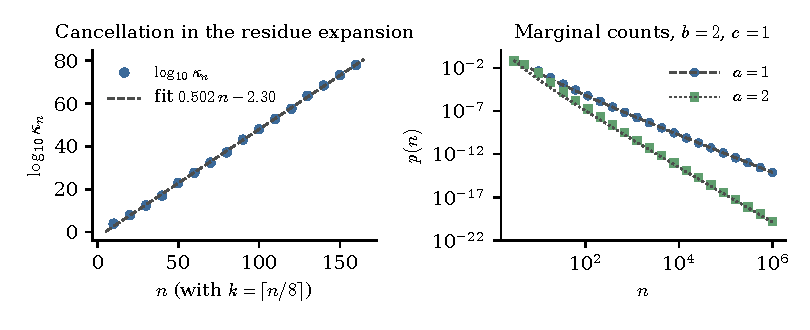
\includegraphics[width=\textwidth]{figures/rc_tails.pdf}
\caption{Left: $\log_{10}\kappa_n$ for the Dirichlet process posterior, the Ewens kernel with $k=\lceil n/8\rceil$ under $\rcPH(0,1,2,1)$, with its least squares line of slope $0.502$ (dashed). Right: marginal counts of the Negative Binomial, Beta, Pochhammer hierarchy, $b=2$, $c=1$ (points, quadrature) against the asymptote of Theorem~\ref{rc:thm:zipf} (dashed for $a=1$, dotted for $a=2$).}\label{rc:fig:tails}
\end{figure}

\begin{definition}\label{rc:def:tph}
$\alpha\sim\rcTPH(m,a,b,c,d,z)$ if $p(\alpha)\propto z^\alpha\alpha^d[\alpha]^m/[c\alpha+a]^b$ on $\alpha\ge0$, $0<z\le1$. More generally, for a polynomial $P$ that is nonnegative on $[0,\infty)$ we write $\alpha\sim\rcTPH(P;a,b,c,z)$ if $p(\alpha)\propto z^\alpha P(\alpha)/[c\alpha+a]^b$, so that $\rcTPH(m,a,b,c,d,z)=\rcTPH(\alpha^d[\alpha]^m;a,b,c,z)$.
\end{definition}

The general form is needed because updating by a Negative Binomial sample multiplies the numerator by $\prod_i[\alpha]^{n_i}$, which is a polynomial of degree $N=\sum_in_i$ but is not $[\alpha]^N$.

\begin{theorem}[Tilted normalizer]\label{rc:thm:tilt}
Let $\lambda=-\log z>0$ and let $P$ be a polynomial. Write the partial fraction expansion
\[
\frac{P(\alpha)}{[c\alpha+a]^b}\;=\;\Pi(\alpha)+\sum_{i=1}^b\frac{\gamma_i}{c\alpha+a+i-1},\qquad\Pi(\alpha)=\sum_k\pi_k\alpha^k,
\]
with the convention of \eqref{rc:eq:pfconv} and poles $-r_i$, $r_i=(a+i-1)/c$. Then
\begin{equation}\label{rc:eq:tilt}
\int_0^\infty z^\alpha\frac{P(\alpha)}{[c\alpha+a]^b}\dd\alpha\;=\;\sum_k\frac{k!\,\pi_k}{\lambda^{k+1}}\;+\;\frac1c\sum_{i=1}^b\gamma_ie^{\lambda r_i}E_1(\lambda r_i),
\end{equation}
where $E_1(x)=\int_x^\infty t^{-1}e^{-t}\dd t$. No degree condition is required: \eqref{rc:eq:tilt} holds for every $b\ge0$, and all moments exist, obtained by replacing $P$ with $\alpha^kP$. As $\lambda\downarrow0$, when $\deg P\le b-2$ so that $\Pi\equiv0$ and $\sum_i\gamma_i=0$, \eqref{rc:eq:tilt} converges to the untilted normalizer $-c^{-1}\sum_i\gamma_i\log r_i$ of Theorems~\ref{rc:thm:residue} and \ref{rc:thm:mellin} via $e^xE_1(x)=-\log x-\rcgE+O(x\log x)$.
\end{theorem}

The intuition is that the tilt $e^{-\lambda\alpha}$ turns each simple pole into an exponential integral, exactly as Laplace transforming $1/(\alpha+r)$ does, and turns each power $\alpha^k$ of the polynomial part into a Gamma integral; nothing else can appear.

The removal of the degree condition matters. In the untilted family, conjugate updating by $\prod_i[\alpha]^{n_i}$ requires $b\ge m+N+2$, so a prior hyperparameter must grow with the total count, which is both awkward to elicit and, by Proposition~\ref{rc:prop:cond}, computationally punishing. With a tilt present, however small, $b$ may be held fixed at the default 2. The scaled function $e^xE_1(x)$ is in every standard library and is stable for all $x>0$; \eqref{rc:eq:tilt} inherits the conditioning of the untilted case and nothing worse.

\begin{corollary}[Tilted distribution function]\label{rc:cor:tiltcdf}
For $\alpha\sim\rcTPH(P;a,b,c,z)$, with the notation of Theorem~\ref{rc:thm:tilt} and $Z$ the right side of \eqref{rc:eq:tilt},
\[
\Prob(\alpha\le A)\;=\;\frac1Z\Bigl[\sum_k\frac{\pi_k\,\gamma_{\mathrm{inc}}(k+1,\lambda A)}{\lambda^{k+1}}+\frac1c\sum_i\gamma_ie^{\lambda r_i}\bigl\{E_1(\lambda r_i)-E_1(\lambda(r_i+A))\bigr\}\Bigr],
\]
where $\gamma_{\mathrm{inc}}(s,x)=\int_0^xt^{s-1}e^{-t}\dd t$ is the lower incomplete Gamma function. This is a monotone function of $A$ computable at the same cost as the normalizer, so exact draws follow by bisection on the uniform scale. When $\Pi\equiv0$ the first sum is absent.
\end{corollary}

\subsection{Global local Pochhammer priors}\label{rc:sec:globallocal}

The half horseshoe is purely local: each $\alpha_k$ gets an independent $\rcPH(0,a,2,c)$. The horseshoe of \citet{rc:carvalho2010} owes much of its performance to the global scale. We therefore set
\[
\alpha_k\mid\tau\;\sim\;\rcPH(0,a,2,c/\tau)\text{ independently},\qquad\tau\sim p(\tau),
\]
so $\alpha_k/\tau$ has the standard shape. Since $c$ enters only through $r_i=(a+i-1)\tau/c$, the conditional of $\tau$ given $\alpha$ is rational whenever $p(\tau)$ is, and each $\alpha_k$ conditional remains in $\rcP$. In the Dirichlet Multinomial the global scale plays the role of the total mass $A=\sum_k\alpha_k$, which is exactly the quantity the heterogeneous Gibbs conditional $p(\alpha_k\mid n_k,N,A_{-k})\propto[\alpha_k]^{n_k}[\alpha_k]^m/\{[\alpha_k+A_{-k}]^N[c\alpha_k+a]^b\}$ couples through. Placing a prior on $\tau$ therefore regularizes the coupling directly rather than through the data alone.

\subsection{Product form}

Definition~\ref{rc:def:class} already permits several denominators, and Theorem~\ref{rc:thm:residue} applies verbatim to $p(\alpha)\propto\alpha^d\prod_j[\alpha+v_j]^{p_j}/\prod_l[c_l\alpha+a_l]^{q_l}$. This matters because, by Proposition~\ref{rc:prop:conj}(iii), a posterior after several rounds of updating is of product form even when the prior was not. Sequential updating is therefore closed but not stationary in the hyperparameters, and the pole set is the right bookkeeping device.

\section{Gamma Shapes and Damsleth's Class}\label{rc:sec:gamma}

\subsection{The class and the obstruction}

Let $x_1,\dots,x_n$ be independent $\rcGa(\alpha,\beta)$. The likelihood is $(\beta^\alpha/\Gamma(\alpha))^n(\prod_ix_i)^{\alpha-1}e^{-\beta\sum_ix_i}$, with sufficient statistic $(n,\sum_ix_i,\prod_ix_i)$. \citet{rc:damsleth1975} studies the natural conjugate class
\begin{equation}\label{rc:eq:damsleth}
p(\alpha,\beta\mid\nu,\rho,\eta)\;\propto\;\Bigl(\frac{\beta^\alpha}{\Gamma(\alpha)}\Bigr)^\nu\rho^\alpha e^{-\eta\beta}\beta^{-1},
\end{equation}
which updates by $(\nu,\rho,\eta)\mapsto(\nu+n,\rho\prod_ix_i,\eta+\sum_ix_i)$ and has $\beta\mid\alpha\sim\rcGa(\nu\alpha,\eta)$, so only the marginal
\begin{equation}\label{rc:eq:damslethmarg}
p(\alpha)\;\propto\;\frac{\Gamma(\nu\alpha)}{\Gamma(\alpha)^\nu}\cdot\frac{\rho^\alpha}{\eta^{\nu\alpha}}
\end{equation}
is problematic. It is the reference point for the modern literature, including the quasiconjugate transfer to generalized Pareto tails and the Gamma approximation of \citet{rc:miller2019}.

\begin{proposition}[The rational boundary]\label{rc:prop:boundary}
$\Gamma(\alpha+u)/\Gamma(\alpha+v)$ is a rational function of $\alpha$ if and only if $u-v\in\mathbb{Z}$.
\end{proposition}

\begin{proof}
If $u-v=k\ge0$ the ratio is $[\alpha+v]^k$, a polynomial, and for $k<0$ a reciprocal polynomial. Conversely the ratio has poles at $\alpha=-u-j$, $j\ge0$, and zeros at $\alpha=-v-j$. These sets are disjoint when $u-v\notin\mathbb{Z}$, so the ratio has infinitely many uncancelled poles, whereas a rational function has finitely many.
\end{proof}

Hence a likelihood lies in $\rcR$ if and only if its Gamma functions appear in ratios whose arguments differ by integers \emph{and} share the same affine function of $\alpha$. The Damsleth marginal \eqref{rc:eq:damslethmarg} fails on both counts: $\Gamma(\nu\alpha)$ and $\Gamma(\alpha)^\nu$ involve different affine maps, and $\Gamma(\alpha)^{-\nu}$ is not a rational function of $\alpha$, so it admits no finite partial fraction expansion. The tilt $\rho^\alpha\eta^{-\nu\alpha}$, by contrast, is harmless: it is exactly the $z^\alpha$ of Theorem~\ref{rc:thm:tilt}. The sole obstruction is $\Gamma(\nu\alpha)/\Gamma(\alpha)^\nu$.

\subsection{Exact repairs}

\paragraph{Lattice shapes.} If $\alpha\in\{\alpha_0+j:j\ge0\}$, as in Erlang and phase type models, then $\Gamma(\alpha)/\Gamma(\alpha_0)=[\alpha_0]^j$ and the likelihood is Pochhammer rational in $j$. A Pochhammer prior on $j$ gives exact conjugate inference for the number of phases, a quantity of direct interest in queueing and reliability.

\paragraph{Poisson augmentation.} The sharpest repair replaces continuous observations by counts. If $\lambda_i\sim\rcGa(\alpha,\beta)$ and $n_i\mid\lambda_i\sim\rcPoi(\lambda_i)$ then $n_i\sim\rcNB(\alpha,\pi)$, $\pi=\beta/(1+\beta)$, and the Gamma functions appear as $\Gamma(\alpha+n_i)/\Gamma(\alpha)$, with integer shift and common argument.

\begin{proposition}[Exact conjugacy for the Gamma shape]\label{rc:prop:gammashape}
In the Gamma Poisson model with $\pi\mid\alpha\sim\rcBe(c\alpha+a,b)$ and $\alpha\sim\rcPH(m,a,b,c)$,
\[
p(\alpha\mid\bm n)\;\propto\;\frac{\prod_k[\alpha]^{n_k}[\alpha]^m}{[(c+K)\alpha+a]^{N+b}}\;\in\;\rcP,
\]
so all normalizers, moments and predictives follow from Theorem~\ref{rc:thm:residue}. If instead $\pi\sim\rcBe(a_0,b_0)$ independently of $\alpha$, then conditionally on $\pi$ the posterior of $\alpha$ is $\rcTPH(P_{\bm n};a,b,c,\pi^K)$ with $P_{\bm n}(\alpha)=[\alpha]^m\prod_k[\alpha]^{n_k}$, exactly, and $\pi\mid\alpha,\bm n\sim\rcBe(K\alpha+a_0,N+b_0)$, giving a two block Gibbs sampler with both blocks drawn exactly.
\end{proposition}

The interpretation is clean: the Gamma shape is learnable in closed form exactly when the information about it arrives through counts. That is not restrictive in the applications motivating Damsleth's class, namely overdispersion, credibility and degradation, where the shape is identified through discrete events.

\paragraph{Tilted approximation.} When continuous Gamma data must be used, \citet{rc:miller2019} shows the full conditional of $\alpha$ is well approximated by a Gamma. A $\rcTPH(0,a,b,c,d,e^{-\lambda})$ retains a heavy body and a pole free tail while matching the Gamma in the tilt; its log derivative is $d/\alpha-\lambda-c\sum_{i=1}^b(c\alpha+a+i-1)^{-1}$, so $(d,\lambda)$ can be matched to the first two log derivatives of \eqref{rc:eq:damslethmarg} at the mode by solving two equations. This yields a proposal or variational family with exact normalizer, not an exact posterior, and we flag it as such.

\paragraph{Reciprocal Gamma augmentation.} The three repairs above all work by altering the model until the likelihood becomes rational. A fourth leaves the model alone and augments instead. \citet{rc:he2019,rc:he2021} attack $1/\Gamma(\alpha)$ head on: building on the classical normal variance mean mixture representations of the reciprocal Gamma function, they construct the P\'olya Inverse Gamma class, and its exponential counterpart, so that conditionally on a latent P\'olya Inverse Gamma variable the shape parameter has a tractable full conditional. Their scheme requires no integer shift and no common affine argument, and so reaches exactly the transcendental factor $\Gamma(\nu\alpha)/\Gamma(\alpha)^\nu$ that Proposition~\ref{rc:prop:boundary} places outside $\rcR$. It applies to Damsleth's class directly.

The relation to the present chapter is complementary rather than competitive, and the division of labour is clean.
\begin{itemize}
\item Residues apply only when the Gamma functions appear in ratios with integer shifts of a common affine argument, but within that range they return exact normalizers, exact moments and exact marginal likelihoods with no latent variables at all.
\item P\'olya Inverse Gamma augmentation carries no restriction on the arguments, and so covers the cases residues cannot, but it returns a Markov chain rather than a closed form, and marginal likelihoods must then be estimated.
\end{itemize}
Where both apply, as for the Dirichlet Multinomial and Negative Binomial models treated by \citet{rc:he2019} and here, the two are naturally used together: augmentation for estimation, residues for the marginal likelihood and for Bayes factors. Section~\ref{rc:sec:exact} is an instance of the same pattern with a different augmentation.

\subsection{The Chinese restaurant table dual}\label{rc:sec:crt}

There is a complementary expansion. The unsigned Stirling numbers of the first kind give
\begin{equation}\label{rc:eq:stirling}
[\alpha]^n=\sum_{\ell=1}^n|s(n,\ell)|\,\alpha^\ell,
\end{equation}
which \citet{rc:zhou2015} exploit as the Chinese restaurant table augmentation: with $\ell\mid n,\alpha\sim\rcCRT(n,\alpha)$, $p(\ell\mid n,\alpha)=|s(n,\ell)|\alpha^\ell/[\alpha]^n$, so $p(\ell,n\mid\alpha)\propto|s(n,\ell)|\alpha^\ell\pi^\alpha$ and a Gamma prior becomes conjugate.

These two devices are duals. Partial fractions expand the \emph{denominator} into simple poles; \eqref{rc:eq:stirling} expands the \emph{numerator} into monomials. Together with the reciprocal Gamma mixtures of \citet{rc:he2019,rc:he2021}, which dissolve the Gamma function itself into a normal variance mean mixture, they make three distinct ways of rendering a Gamma ratio tractable. The tradeoffs of the first two are opposite:
\begin{itemize}
\item Stirling: all terms positive, perfectly conditioned, but $O(N^2)$ enormous integers and, being an augmentation, a Markov chain rather than a closed form.
\item Residues: closed form, no auxiliary variables, exact moments and marginal likelihoods, but ill conditioned by Proposition~\ref{rc:prop:cond}.
\end{itemize}

The hybrid is obvious and we recommend it: residues for marginal likelihoods and Bayes factors, where one accurate number is wanted; CRT augmentation inside long chains, where stability over millions of iterations matters. Equating the two expansions of $\int_0^\infty[\alpha]^n\{[c\alpha+a]^b\}^{-1}\dd\alpha$ gives, for $b\ge n+2$,
\[
\sum_{\ell=1}^n|s(n,\ell)|\,\rcM_{0,a,b,c}(\ell+1)\;=\;-\frac1c\sum_{i=1}^b\gamma_i^{(n,a,b,c)}\log\frac{a+i-1}{c},
\]
a signed sum of residues written as a positive combination of Mellin values.

\section{The Negative Binomial Family}\label{rc:sec:nb}

\subsection{The induced count distribution is a power law}

\citet{rc:wang2024} couple $\pi$ to $\alpha$ via $\pi\mid\alpha\sim\rcBe(c\alpha+a,b)$ for joint conjugacy, and display the resulting sparsity patterns numerically. The construction in fact determines the marginal law of the counts exactly, and it is a Zipf law.

\begin{theorem}[Zipf tails]\label{rc:thm:zipf}
Let $\alpha\sim\rcPH(m,a,b,c)$ with normalized density $p_\alpha$, $\pi\mid\alpha\sim\rcBe(c\alpha+a,b)$ and $n\mid\alpha,\pi\sim\rcNB(\alpha,\pi)$. Then as $n\to\infty$
\begin{equation}\label{rc:eq:zipf}
\begin{gathered}
p(n)\;\sim\;K\,n^{-(1+a)}(\log n)^{-(1+\iota)},\\
K=\frac{\Gamma(a)\,\Gamma(1+\iota)\,\varpi}{B(a,b)\,c^{1+\iota}},\qquad \iota=1+\rcone(m\ge1),
\end{gathered}
\end{equation}
where $\varpi=\lim_{\alpha\downarrow0}\alpha^{-\rcone(m\ge1)}p_\alpha(\alpha)$. For the default $m=0$, $\iota=1$ and the tail is $Kn^{-(1+a)}(\log n)^{-2}$ with $K=\Gamma(a)p_\alpha(0)/\{B(a,b)c^2\}$; for every $m\ge1$, $\iota=2$ and the correction is $(\log n)^{-3}$. The indicator, rather than $m$ itself, appears because $[\alpha]^m$ vanishes only to first order at the origin.
\end{theorem}

The proof, given at the end of the chapter, is Watson's lemma: $p(n\mid\alpha)\sim\rcK(\alpha)n^{-c\alpha-a-1}$ with $\rcK(\alpha)\to\alpha\Gamma(a)/B(a,b)$ as $\alpha\downarrow0$, so the integral over $\alpha$ concentrates on a neighbourhood of the origin of width $1/(c\log n)$, and the order of vanishing of $\rcK p_\alpha$ at the origin, namely $\iota$, produces the power of the logarithm.

Three consequences. The tail exponent is the prior hyperparameter $a$ alone; $b$ and $c$ affect only the constant, and $m$ only the logarithmic correction. At the default $a=1,b=2,c=1,m=0$ one gets $p(n)\asymp n^{-2}(\log n)^{-2}$, so $\E(n)<\infty$ and $\E(n^2)=\infty$, the standard regime for word frequencies, degrees and claim severities, obtained without any explicit power law modelling. And the mechanism is transparent: the zero of $\Gamma(\alpha)^{-1}$ at the origin together with nondecaying prior mass near zero converts geometric decay into polynomial decay. Excess zeros and Zipf tails are two faces of the same prior mass at $\alpha=0$. This is the count model form of the quasisparsity that motivated \citet{rc:datta2016}, and it is the analytic content of Figure 3 of \citet{rc:wang2024}. The right panel of Figure~\ref{rc:fig:tails} verifies \eqref{rc:eq:zipf} to $n=10^6$; convergence to $K$ is $O(1/\log n)$, as the argument predicts.

\subsection{Negative Binomial regression: P\'olya Gamma meets Pochhammer}

Let $n_i\sim\rcNB(\alpha,\pi_i)$ with $\psi_i=\log\{(1-\pi_i)/\pi_i\}=\bm x_i^\top\bm\beta$, so that
\[
p(n_i\mid\alpha,\bm\beta)=\frac{[\alpha]^{n_i}}{n_i!}\,\frac{(e^{\psi_i})^{n_i}}{(1+e^{\psi_i})^{n_i+\alpha}}.
\]
\citet{rc:polson2013} give $(e^\psi)^n(1+e^\psi)^{-(n+\alpha)}=2^{-(n+\alpha)}e^{\kappa\psi}\E_\omega\{e^{-\omega\psi^2/2}\}$ with $\kappa=(n-\alpha)/2$ and $\omega\sim\rcPG(n+\alpha,0)$, so $\bm\beta\mid\bm\omega$ is Gaussian. The obstruction has always been $\alpha$, which appears both in $[\alpha]^{n_i}$ and in the P\'olya Gamma \emph{index}. \citet{rc:he2019} resolve it by a P\'olya Inverse Gamma draw for $\alpha$; we resolve it differently, and without leaving the prior family. The index dependence is not rational and cannot be handled by conditioning on $\bm\omega$. It can be handled by not conditioning on $\bm\omega$ at all.

\begin{proposition}[Exact dispersion block]\label{rc:prop:dispersion}
Marginally in $\bm\omega$,
\[
p(\alpha\mid\bm n,\bm\beta)\;\propto\;\prod_{i=1}^K[\alpha]^{n_i}\pi_i^\alpha\,p(\alpha)\;=\;\prod_i[\alpha]^{n_i}z^\alpha p(\alpha),\qquad z=\prod_{i=1}^K\frac{1}{1+e^{\psi_i}},
\]
so with $p=\rcPH(m,a,b,c)$ one has $\alpha\mid\bm n,\bm\beta\sim\rcTPH(P_{\bm n};a,b,c,z)$, $P_{\bm n}(\alpha)=[\alpha]^m\prod_i[\alpha]^{n_i}$, exactly, for \emph{any} $b\ge0$, with $\lambda=\sum_i\log(1+e^{\psi_i})$. Drawing $\alpha$ from this law before redrawing $\bm\omega$ gives a partially collapsed Gibbs sampler with the correct stationary distribution.
\end{proposition}

Algorithm 1 records the sampler. It is blocked, free of Metropolis steps, and the ordering matters: $\bm\omega$ must be redrawn after $\alpha$ and before $\bm\beta$, in the manner of \citet{rc:vandyk2008}; reversing the order targets the wrong distribution. Theorem~\ref{rc:thm:tilt} is what makes the $\alpha$ block exact, and its removal of the degree condition is what keeps $b$ fixed at 2 rather than growing with $N$. For large $N$ the residue draw may be replaced by a CRT draw, per Section~\ref{rc:sec:crt}, without changing the target.

Zero inflation needs no mixture component: when many $n_i$ vanish the tilted posterior retains its concentration at the origin, which is Remark 4 of \citet{rc:wang2024} in the presence of covariates.

\begin{center}
\begin{minipage}{\textwidth}
\small
\hrule height 0.8pt\smallskip
\textsc{Algorithm 1}\enspace Negative Binomial regression with Pochhammer dispersion
\smallskip\hrule\smallskip
\begin{enumerate}[label={\footnotesize\arabic*:},leftmargin=1.8em,itemsep=1pt,topsep=0pt]
\item Input counts $\bm n$, design $X$, prior $\rcPH(m,a,b,c)$ on $\alpha$, $\bm\beta\sim N(0,B)$
\item for $t=1,\dots,T$ do
\item \hspace{1em}$\psi_i\leftarrow\bm x_i^\top\bm\beta$;\ \ $\lambda\leftarrow\sum_i\log(1+e^{\psi_i})$
\item \hspace{1em}$\alpha\sim\rcTPH(P_{\bm n};a,b,c,e^{-\lambda})$\hfill$\triangleright$ exact, by Corollary~\ref{rc:cor:tiltcdf}; $\bm\omega$ marginalized
\item \hspace{1em}$\omega_i\sim\rcPG(n_i+\alpha,\psi_i)$, $i=1,\dots,K$
\item \hspace{1em}$\bm\beta\sim N(\Sigma X^\top\bm\kappa,\Sigma)$, $\Sigma=(X^\top\Omega X+B^{-1})^{-1}$, $\kappa_i=(n_i-\alpha)/2$
\end{enumerate}
\smallskip\hrule height 0.8pt
\end{minipage}
\end{center}

\begin{center}
\begin{minipage}{\textwidth}
\small
\hrule height 0.8pt\smallskip
\textsc{Algorithm 2}\enspace Negative Binomial regression, half horseshoe dispersion, all blocks exact
\smallskip\hrule\smallskip
\begin{enumerate}[label={\footnotesize\arabic*:},leftmargin=1.8em,itemsep=1pt,topsep=0pt]
\item Input counts $\bm n$, design $X$, prior $\rcPH(0,a,b,c)$ with poles $r_i=(a+i-1)/c$, $\bm\beta\sim N(0,B)$
\item for $t=1,\dots,T$ do
\item \hspace{1em}$\ell_i\sim\rcCRT(n_i,\alpha)$,\ $L\leftarrow\sum_i\ell_i$\hfill$\triangleright$ $\ell_i=\sum_{j=1}^{n_i}\mathrm{Bern}\{\alpha/(\alpha+j-1)\}$
\item \hspace{1em}$\tau\leftarrow\sum_{i=1}^bE_i$ with $E_i\sim\rcExp(r_i+\alpha)$ independent\hfill$\triangleright$ $b=2$ at the default prior
\item \hspace{1em}$\psi_i\leftarrow\bm x_i^\top\bm\beta$,\ $\lambda\leftarrow\sum_i\log(1+e^{\psi_i})$
\item \hspace{1em}$\alpha\sim\rcGa(L+1,\,\lambda+\tau)$
\item \hspace{1em}$\omega_i\sim\rcPG(n_i+\alpha,\psi_i)$;\ $\bm\beta\sim N(\Sigma X^\top\bm\kappa,\Sigma)$, $\Sigma=(X^\top\Omega X+B^{-1})^{-1}$, $\kappa_i=(n_i-\alpha)/2$
\end{enumerate}
\smallskip\hrule height 0.8pt
\end{minipage}
\end{center}

\subsection{An exact sampler with no ill conditioning}\label{rc:sec:exact}

Algorithm 1 draws $\alpha$ from a tilted law whose numerator $P_{\bm n}$ has degree $m+N$. Its pole set does not grow, but dividing $P_{\bm n}$ by $[c\alpha+a]^b$ to obtain the polynomial part is a long signed recursion of the same kind as the residue sums of Proposition~\ref{rc:prop:cond}, and it too loses digits: for $K=40$ counts with $N=59$ under $\rcPH(0,\frac12,2,1)$ and $\lambda=40\log2$, the normalizer \eqref{rc:eq:tilt} is $53.8513331487$, but computed with sixteen significant digits it comes out negative, and about thirty digits are needed for twelve correct ones. Extended precision is therefore required once $N$ is large. Theorem~\ref{rc:thm:cm} removes the difficulty at the default prior. Augmenting by $\tau$ turns the prior into a tilt, and augmenting by the Chinese restaurant tables turns $\prod_i[\alpha]^{n_i}$ into a monomial, so the two devices of Section~\ref{rc:sec:crt} combine into a sampler in which every block is an exact standard draw.

Write $\lambda=\sum_i\log(1+e^{\psi_i})$, so that $\prod_i\pi_i^\alpha=e^{-\lambda\alpha}$. Conditionally on the tables $\ell_i$ and on $\tau$,
\[
p(\alpha\mid\bm\ell,\tau,\bm\beta)\;\propto\;\alpha^Le^{-(\lambda+\tau)\alpha},\qquad L=\sum_i\ell_i,
\]
which is $\rcGa(L+1,\lambda+\tau)$. Conditionally on $\alpha$, the latent scale has the closed form distribution function of Proposition~\ref{rc:prop:plugin}. Proposition~\ref{rc:prop:dispersion} supplies the remaining block, and Algorithm 2 is the result.

Every step is an exponential, Gamma, Bernoulli, Gaussian or P\'olya Gamma draw. No residue is computed anywhere, so Proposition~\ref{rc:prop:cond} is irrelevant however large $N$ becomes, and the sampler is exact in the sense that each block is drawn from its full conditional without approximation. The price is two latent variables in place of one closed form draw, together with the usual loss of the marginal likelihood: Algorithm 1 returns $p(\bm n)$ as a byproduct and Algorithm 2 does not. Use Algorithm 2 for estimation and Algorithm 1, at extended precision, for model comparison.

As a check we ran Algorithm 2 on $K=40$ counts drawn from $\rcNB(1.7,\tfrac12)$ under $\rcPH(0,1,2,1)$, with no covariates so that the exact posterior is available by quadrature. Five chains of $1.2\times10^5$ draws give posterior mean $1.6026$ and $95\%$ interval $(1.127,2.152)$, against the exact $1.6031$ and $(1.126,2.154)$; the discrepancy is within two Monte Carlo standard errors of $3\times10^{-4}$.

\subsection{Waring and Beta Negative Binomial}\label{rc:sec:waring}

For integer $r$,
\[
p(n\mid r,\alpha,\rho)=\frac{[r]^n}{n!}\,\frac{B(\alpha+r,\rho+n)}{B(\alpha,\rho)}=\frac{[r]^n}{n!}\cdot\frac{[\rho]^n[\alpha]^r}{[\alpha+\rho]^{n+r}},
\]
Pochhammer rational in $\alpha$, in $\rho$ and in $r$ separately. Setting $r=1$ gives Waring, and the further choice $\rho=1$ makes $n+1$ Yule Simon with parameter $\alpha$. Pochhammer priors on $\alpha$ and $\rho$, and a lattice Pochhammer prior on $r$, give a fully conjugate three parameter analysis by Gibbs. Since the tail index of the Beta Negative Binomial is $\alpha$, this is a second and more direct route to a learnable power law, complementary to Theorem~\ref{rc:thm:zipf}: there the exponent is a hyperparameter, here it is a parameter with a conjugate posterior.

\section{Examples in Applied Probability}\label{rc:sec:examples}

This section runs through the likelihoods of Table~\ref{rc:tab:members} one at a time, to show what the general theory delivers in each and where its limits lie. The Ewens and Pitman Yor cases, which matter most for genetics, are introduced here and worked through numerically in Section~\ref{rc:sec:genetics}.

\subsection{P\'olya urns and reinforcement}\label{rc:sec:urn}

An urn holds $a$ white and $\beta$ black; a drawn ball is returned with one of the same colour. After $n$ draws with $k$ white, $\Prob=\binom nk[a]^k[\beta]^{n-k}/[a+\beta]^n$, the Beta Binomial law, rational in $a$ for fixed $\beta$ and conversely. With experiments $(n_i,k_i)$,
\[
p(a\mid\text{data})\;\propto\;\frac{[a]^m\prod_i[a]^{k_i}}{[c_0a+a_0]^{b_0}\prod_i[a+\beta]^{n_i}},
\]
with poles at $-(a_0+j-1)/c_0$ and at $-(\beta+j)$ of multiplicity $\#\{i:n_i>j\}$, so Theorem~\ref{rc:thm:residue} is needed as soon as two experiments overlap. The quantity of interest is usually the limiting white fraction $W_\infty\sim\rcBe(a,\beta)$, and $\E\{a/(a+\beta)\mid\text{data}\}$ is again a ratio of normalizers. This delivers uncertainty quantification for the strength of reinforcement, which the exchangeable urn literature typically fixes by fiat.

\subsection{Ewens, cycles and the Feller coupling}\label{rc:sec:ewens}

Under the Ewens sampling formula \citep{rc:ewens1972} only $\theta^k/[\theta]^n$ depends on $\theta$, so the number of alleles $k$ is sufficient and the likelihood is Pochhammer rational. Under the Feller coupling, $k=\sum_{i=1}^n\xi_i$ with independent $\xi_i\sim\mathrm{Bern}\{\theta/(\theta+i-1)\}$, whence the Fisher information is
\[
I_n(\theta)=\sum_{i=1}^n\frac{i-1}{\theta(\theta+i-1)^2}\;\sim\;\frac{\log n}{\theta},
\]
so $\hat\theta_n$ is asymptotically $N(\theta,\theta/\log n)$: the effective sample size is $\log n$. Uncertainty quantification therefore matters more here than almost anywhere, and a point estimate is close to useless. It also means the likelihood is too flat to overcome a light tailed prior, so the heavy tail of Corollary~\ref{rc:cor:tail} is a necessity rather than a luxury.

Two further payoffs. The one step predictive probability of a new block is $\Prob(\xi_{n+1}=1\mid k)=\E\{\theta/(\theta+n)\mid k\}$, a ratio of two normalizers in $\rcP$, since multiplying the posterior kernel by $\theta/(\theta+n)$ raises the numerator degree by one and adjoins a pole at $-n$. Sequential prediction is thus exact and simulation free, which matters in streaming settings. And the case $\theta=1$ is the uniform random permutation, for which $k$ is the number of cycles with $\E k=\log n+\rcgE+o(1)$, so the same formulas give exact posterior inference for the reinforcement of a Chinese restaurant process from a single observation of the block count.

\subsection{Dirichlet process and Pitman Yor concentration}\label{rc:sec:py}

For a Dirichlet process mixture, $p(K_n=k\mid\theta)=|s(n,k)|\theta^k/[\theta]^n$, the Ewens likelihood again. \citet{rc:escobar1995} introduce a Beta auxiliary variable so that a Gamma prior is conditionally conjugate, at the cost of a latent variable and a two component Gamma mixture. The Pochhammer prior removes the auxiliary variable and returns the exact marginal posterior and its moments; Example~\ref{rc:ex:double} is the calculation.

The Stirling gamma distribution of \citet{rc:zito2024} has a similar functional form and was built for exactly this problem. The two lines of work are independent, as \citet{rc:wang2024} record, and \citet{rc:zito2024} appeared first, in June 2023. The underlying device is older than either: the partial fraction and residue calculus applied here to Gamma ratios is the one used for the integrals in \citet{rc:polson2013}, and Section 2.2 of \citet{rc:wang2024} identifies that lineage explicitly. On the Dirichlet process itself the Stirling gamma is the better instrument, being designed for that problem, having hyperparameters with a direct partition interpretation, and coming with an efficient rejection sampler and a careful treatment of elicitation through the induced law of the number of clusters.

What the Pochhammer view adds is scope rather than a better answer to the same question. Stirling gamma conjugacy for the partition requires one hyperparameter to be tied to the sample size $n$, whereas Proposition~\ref{rc:prop:conj} gives closure for the whole rational class $\rcR$ with no such tie, so a single theorem covers the Dirichlet Multinomial, Negative Binomial, urn, Waring and Erlang likelihoods as well. Three further items are new here: repeated and complex poles in Theorem~\ref{rc:thm:residue}, which the Pitman Yor case immediately below forces; the Mellin transform and its corollaries; and the exponential mixture of Theorem~\ref{rc:thm:cm}, which yields the sampler of Section~\ref{rc:sec:exact}.

For $\mathrm{PY}(\sigma,\theta)$ with $0\le\sigma<1$, $\theta>-\sigma$, the exchangeable partition probability function is \citep{rc:pitman2006}
\[
p(\text{partition})=\frac{\prod_{i=1}^{k-1}(\theta+i\sigma)}{[\theta+1]^{n-1}}\prod_{j=1}^k[1-\sigma]^{n_j-1},
\]
so for fixed $\sigma$ the likelihood in $\theta$ depends on the data only through $(n,k)$ and is rational of numerator degree $k-1$ and denominator degree $n-1$, with poles at $-1,\dots,-(n-1)$. Combined with a prior $\rcPH(0,a,b,c)$, $b\ge2$, the posterior has numerator degree $k-1$ and denominator degree $n-1+b\ge k+1$, so it is proper for every $k\le n$ and the prior is exactly conjugate. We restrict to $\theta\ge0$, the part of the parameter space $\theta>-\sigma$ on which the Pochhammer prior lives. A prior pole $-(a+i-1)/c$ coincides with a likelihood pole when $(a+i-1)/c\in\{1,\dots,n-1\}$, for instance for every $i$ when $c=1$ and $a$ is a positive integer, and the posterior then has double poles; otherwise all poles are simple. The numerator roots $-i\sigma$, $1\le i\le k-1$, lie on the negative axis among the poles, and when $i\sigma$ is an integer a root cancels a pole outright; at $\sigma=\frac12$, for example, every second root does so. This interplay between $\sigma$ and the pole set is one analytic expression of the known weak identifiability of $(\sigma,\theta)$ from the block count. Conditionally on $\theta$, the likelihood in $\sigma$ is a polynomial but lies outside $\rcR$, because $[1-\sigma]^{n_j-1}$ violates the sign condition $u_j\ge0$ of Definition~\ref{rc:def:class}, so we recommend an exact residue draw for $\theta$ and a griddy or Metropolis step for $\sigma$. The exact marginal likelihood in $\theta$ also permits model choice among nonparametric priors by Bayes factor rather than by predictive check.

\subsection{Yule processes, preferential attachment and Zipf}\label{rc:sec:yule}

A linear birth process of rate $\lambda$ per individual with new types arriving at rate $\mu$ per existing type gives, at stationarity, the Yule Simon law \citep{rc:simon1955}, $p(n\mid\rho)=\rho B(n,\rho+1)$, with $\rho=\mu/\lambda$, so the likelihood over $K$ observations is $\rho^K/\prod_k[\rho+1]^{n_k}$, Pochhammer rational. Here $\rho$ is both the scientific quantity in preferential attachment models of citation, degree and firm size, and the power law exponent, $p(n\mid\rho)\sim\rho\,\Gamma(\rho+1)\,n^{-(1+\rho)}$. A Pochhammer prior therefore yields the exact posterior of a power law exponent from raw counts, in contrast to the Hill estimator and to discrete maximum likelihood, neither of which propagates exponent uncertainty into predictions.

\begin{proposition}[Boundary Zipf law]\label{rc:prop:boundaryzipf}
Under $\rho\sim\rcPH(0,a,b,c)$ with density $p_\rho$, the Yule Simon prior predictive satisfies $p(n)\sim p_\rho(0)\,n^{-1}(\log n)^{-2}$ as $n\to\infty$. This is a proper distribution, since $\sum_nn^{-1}(\log n)^{-2}<\infty$, but it has no moments of any positive order.
\end{proposition}

The exponent one is the boundary of summability, reached only because of the logarithmic correction. This is the count model analogue of the horseshoe sitting exactly at the boundary of integrability, and it is the sense in which the half horseshoe is the least informative proper prior for a Zipf exponent.

\subsection{Insurance claim counts and credibility}

The Gamma Poisson mixture is the classical credibility model: policyholder $i$ has latent frequency $\lambda_i\sim\rcGa(\alpha,\beta)$ and count $n_i\sim\rcPoi(\lambda_it_i)$. B\"uhlmann credibility replaces the posterior mean of $\lambda_i$ by a linear estimate with $\alpha$ plugged in from moments or maximum likelihood. Proposition~\ref{rc:prop:gammashape} makes the exact Bayesian treatment available, so the credibility factor $Z_i=t_i/(t_i+\beta)$ becomes a random variable with a computable distribution rather than a constant. The heavy prior tail of Corollary~\ref{rc:cor:tail} means the data may push $\alpha$ to large values, that is towards Poisson behaviour, without prior resistance, and the excess zeros normal in motor and health portfolios are handled by the mass at the origin rather than by a zero inflation mixture. Covariates enter through Algorithm 1.

\subsection{Erlang's loss formula and complex poles}\label{rc:sec:erlang}

For $c$ trunks with offered load $A$ and no waiting room, the stationary blocking probability is $B(c,A)=(A^c/c!)/\sum_{j=0}^cA^j/j!$, rational in $A$. Observing $y$ blocked calls among $M$ offered gives the Binomial likelihood $B(c,A)^y\{1-B(c,A)\}^{M-y}$. Since $1-B(c,A)=\sum_{j<c}(A^j/j!)/\sum_{j\le c}A^j/j!$, this is rational with numerator degree $cy+(c-1)(M-y)\le cM$ and denominator degree $cM$, so any proper rational prior yields a proper rational posterior. The poles are the zeros of the truncated exponential $\sum_{j\le c}A^j/j!$. Its coefficients are positive, so none lies on $[0,\infty)$, which is all Theorem~\ref{rc:thm:residue} requires; for even $c$ none is real and for odd $c$ exactly one is, so complex poles are the rule, and by Szeg\H{o}'s theorem the rescaled zeros $A/c$ approach the Szeg\H{o} curve $|ze^{1-z}|=1$, $|z|\le1$, as $c$ grows. For $c=4$ the zeros are $-1.7294\pm0.8890i$ and $-0.2706\pm2.5048i$, all in the left half plane, but from $c=5$ onwards some lie in the right half plane (the largest real part is $0.2398$ at $c=5$ and $3.3749$ at $c=10$), so the poles of a rational likelihood need not lie where those of a Pochhammer factor do. Theorem~\ref{rc:thm:residue} covers this, each conjugate pair contributing $-2\operatorname{Re}\{\gamma\log r\}$, and delivers the exact posterior of the offered load and the exact predictive blocking probability. We are not aware of a previous closed form Bayesian treatment of Erlang's formula. The example also makes the general point that rational conjugacy is not about Gamma ratios: any rational likelihood will do, and Gamma ratios are simply the commonest source of them.

\subsection{Contingency tables and species sampling}

Two examples from \citet{rc:wang2024} extend directly. For multiway tables with $K=4^p$ cells, the heterogeneous half horseshoe places posterior mass near zero for the overwhelming majority of empty cells, and Cram\'er association statistics inherit valid credible intervals. For species sampling, the discovery probability after $n$ observations is $\theta/(\theta+n)$ under the Dirichlet process, so Section~\ref{rc:sec:py} gives an exact posterior for the probability of a new species, the quantity at issue in the Good and Turing literature.

\section{The Ewens Concentration Parameter: Worked Examples}\label{rc:sec:genetics}
\sectionmark{Worked Examples in Genetics}

This section carries the general results through, with actual numbers, on the problem that motivates the book: inference for the scaled mutation rate $\theta$ from a sample of genes classified by allele. We begin with the urn that generates the data, then do one posterior completely by hand, vary the model to Pitman Yor, give an exact sampler, and finish with a classical data set large enough to show both the value of the heavy tail and the cost of the residue formula.

\subsection{The Hoppe urn}

\citet{rc:hoppe1984} gave the Ewens sampling formula a sequential description. An urn holds one black ball of weight $\theta$ and coloured balls of weight one. At each step a ball is drawn with probability proportional to its weight. If it is black, it is returned together with one ball of a colour never seen before, a new allele; otherwise it is returned together with one more ball of its own colour, a copy of an existing allele. The $i$th gene is therefore new with probability $\theta/(\theta+i-1)$, independently of the past, which is the Feller coupling of Section~\ref{rc:sec:ewens}. Multiplying the conditional probabilities along any sequence that ends with $k$ alleles of sizes $n_1,\dots,n_k$ gives
\[
\frac{\theta^k\prod_{j=1}^k(n_j-1)!}{\theta(\theta+1)\cdots(\theta+n-1)}\;=\;\frac{\theta^k}{[\theta]^n}\prod_{j=1}^k(n_j-1)!,
\]
since each allele contributes one factor $\theta$ when it is founded and the factors $1,2,\dots,n_j-1$ as it grows. Summing over sequences gives the Ewens sampling formula $n!\,[\theta]^{-n}\prod_j(\theta/j)^{a_j}/a_j!$ for the allele frequency spectrum $(a_1,\dots,a_n)$, and summing further gives $\Prob(K_n=k\mid\theta)=|s(n,k)|\,\theta^k/[\theta]^n$. In every form $\theta$ enters only through $\theta^k/[\theta]^n$, so $K_n$ is sufficient, and after cancelling one factor $\theta$ the likelihood is $\theta^{k-1}/[\theta+1]^{n-1}$, the kernel $\rcPPH(0,1,n-1,1,k-1)$ of Proposition~\ref{rc:prop:cond}. The Hoppe urn is a P\'olya urn of the kind in Section~\ref{rc:sec:urn} with an immigrant colour, and $\theta$ is its reinforcement parameter.

\subsection{Residues by hand: four genes, two alleles}

The smallest case that shows every feature of Theorem~\ref{rc:thm:residue}, double poles included, is a sample of $n=4$ genes carrying $K_4=2$ alleles, analysed under the half horseshoe $\rcPH(0,1,2,1)$, whose density is $\{(\theta+1)(\theta+2)\log2\}^{-1}$.

\begin{example}[Four genes, two alleles]\label{rc:ex:four}
The posterior kernel is
\[
R(\theta)\;=\;\frac{\theta^2}{\theta(\theta+1)(\theta+2)(\theta+3)}\cdot\frac{1}{(\theta+1)(\theta+2)}\;=\;\frac{\theta}{(\theta+1)^2(\theta+2)^2(\theta+3)},
\]
with double poles at $-1$, $-2$ and a simple pole at $-3$. For the double pole at $-1$ put $h(\theta)=(\theta+1)^2R(\theta)=\theta/\{(\theta+2)^2(\theta+3)\}$. Then $\gamma_{12}=h(-1)=-\frac12$, and since $h'/h=1/\theta-2/(\theta+2)-1/(\theta+3)$ equals $-\frac72$ at $\theta=-1$, $\gamma_{11}=h'(-1)=\frac74$. The same computation at $-2$ gives $\gamma_{22}=-2$, $\gamma_{21}=-1$, and at $-3$, $\gamma_{31}=-3/\{(-2)^2(-1)^2\}=-\frac34$. Hence
\[
R(\theta)=\frac{7/4}{\theta+1}-\frac{1/2}{(\theta+1)^2}-\frac{1}{\theta+2}-\frac{2}{(\theta+2)^2}-\frac{3/4}{\theta+3},
\]
and the check $\sum_i\gamma_{i1}=\frac74-1-\frac34=0$ passes. Formula \eqref{rc:eq:residue} gives the normalizing constant
\[
\begin{aligned}
C\;&=\;-\Bigl(\tfrac74\log1-\log2-\tfrac34\log3\Bigr)-\frac{1/2}{1}-\frac{2}{2}\\
&=\;\log2+\tfrac34\log3-\tfrac32\;=\;0.0171063971.
\end{aligned}
\]
Multiplying the kernel by $\theta$ and repeating the computation gives the coefficients $(-\frac94,\frac12)$ at $-1$, $(0,4)$ at $-2$ and $\frac94$ at $-3$, so $\int_0^\infty\theta R=\frac52-\frac94\log3=0.0281223505$ and the posterior mean is
\[
\E(\theta\mid K_4=2)\;=\;\frac{\frac52-\frac94\log3}{\log2+\frac34\log3-\frac32}\;=\;1.64397.
\]
Similarly $\int_0^\infty\theta^2R=\frac{27}4\log3-4\log2-\frac92$, so $\E(\theta^2\mid K_4=2)=8.36203$ and the posterior standard deviation is $2.37895$. The posterior has no third moment, since $\theta^3R(\theta)\sim\theta^{-1}$. Integrating the partial fractions from $0$ to $A$ gives the distribution function in closed form, and bisection on it gives the posterior median $1.0153$ and the equal tailed $95\%$ interval $(0.1144,\,6.9330)$. Every one of these numbers agrees with adaptive quadrature of $R$ to the ten digits we carried.
\end{example}

The interval is wide, as it must be: four genes carry almost no information about $\theta$, and Figure~\ref{rc:fig:ewens}(a) shows that the posterior differs from the prior mainly by removing mass near zero, where two alleles in four genes would be improbable. The quantity a geneticist is most likely to want is predictive.

\begin{example}[Probability that the next gene is a new allele]\label{rc:ex:pred}
By the Hoppe urn the fifth gene is a new allele with probability $\theta/(\theta+4)$, so the posterior predictive probability is $\E\{\theta/(\theta+4)\mid K_4=2\}$, the ratio of $\int_0^\infty\theta R(\theta)(\theta+4)^{-1}\dd\theta$ to $C$. The new kernel $\theta^2/\{(\theta+1)^2(\theta+2)^2(\theta+3)(\theta+4)\}$ has the coefficients $(-\frac{29}{36},\frac16)$ at $-1$, $(-1,2)$ at $-2$, $\frac94$ at $-3$ and $-\frac49$ at $-4$; the simple residues again sum to zero, and
\[
\Prob(\text{gene 5 is new}\mid K_4=2)\;=\;\frac{\frac76+\frac{17}9\log2-\frac94\log3}{\log2+\frac34\log3-\frac32}\;=\;0.23775.
\]
For comparison, the maximum likelihood estimate solves $\E_\theta K_4=\sum_{i=0}^3\theta/(\theta+i)=2$, giving $\hat\theta=0.8794$ and the plug in probability $\hat\theta/(\hat\theta+4)=0.1802$. The Bayesian answer is about a third larger. The reason is not Jensen's inequality, which for the concave map $\theta\mapsto\theta/(\theta+4)$ pushes the other way, but the shape of the posterior: it is strongly right skewed, with median $1.02$ and mean $1.64$ against $\hat\theta=0.88$, and the plug in value ignores exactly the uncertainty that Section~\ref{rc:sec:ewens} says dominates this problem.
\end{example}

\begin{example}[Prior predictive law of the allele count]\label{rc:ex:priorpred}
Before any data are seen, the half horseshoe induces a law on $K_4$ through $\Prob(K_4=k)=|s(4,k)|\int_0^\infty\theta^k[\theta]^{-4}p(\theta)\dd\theta$, with $|s(4,k)|=6,11,6,1$ for $k=1,\dots,4$. Each integral is a residue sum of the kind just computed. The result, against the uniform random permutation $\theta=1$, is
\begin{center}
\small
\begin{tabular}{@{}lcccc@{}}
\toprule
 & $K_4=1$ & $K_4=2$ & $K_4=3$ & $K_4=4$\\
\midrule
$\theta\sim\rcPH(0,1,2,1)$ & 0.2787 & 0.2715 & 0.2434 & 0.2064\\
$\theta=1$ & 0.2500 & 0.4583 & 0.2500 & 0.0417\\
\bottomrule
\end{tabular}
\end{center}
The half horseshoe spreads its predictive mass almost evenly over the four possible allele counts, from a monomorphic sample to one in which every gene is distinct. This is the sense in which it is uninformative about diversity, and it is a more useful description for elicitation than any statement about the density of $\theta$ itself. The marginal likelihood of the observed $K_4=2$, namely $0.2715=11C/\log2$, is the quantity a Bayes factor between priors would use.
\end{example}

\subsection{The Pitman Yor variant}

The Pitman Yor model adds a discount $\sigma\in[0,1)$ under which the probability of a new type after $n$ draws with $k$ types is $(\theta+k\sigma)/(\theta+n)$, so that types are founded at a rate that grows with their number; $\sigma=0$ is Ewens. Section~\ref{rc:sec:py} showed that for fixed $\sigma$ the likelihood in $\theta$ is again rational.

\begin{example}[Four genes, two types, $\sigma=\frac12$]\label{rc:ex:py}
With $n=4$, $k=2$ the likelihood is $(\theta+\frac12)/\{(\theta+1)(\theta+2)(\theta+3)\}$, and under $\rcPH(0,1,2,1)$ the posterior kernel is $(\theta+\frac12)/\{(\theta+1)^2(\theta+2)^2(\theta+3)\}$, the double pole integrand in the first line of Table~\ref{rc:tab:verify}. Its partial fractions are
\[
\frac{9/8}{\theta+1}-\frac{1/4}{(\theta+1)^2}-\frac{1/2}{\theta+2}-\frac{3/2}{(\theta+2)^2}-\frac{5/8}{\theta+3},
\]
so $C=\frac12\log2+\frac58\log3-1=0.0332062707$. The posterior mean of $\theta$ is $1.1045$ and its median $0.5893$, both well below their Ewens values $1.6440$ and $1.0153$, while the predictive probability of a new type at the fifth draw, $\E\{(\theta+1)/(\theta+4)\mid\text{data}\}$, rises to $0.37867$ from $0.23775$. Part of the novelty that Ewens must attribute to $\theta$ is carried here by $\sigma$, so $\theta$ is smaller, but the discount adds its own contribution $k\sigma/(\theta+n)$ to the predictive. Figure~\ref{rc:fig:ewens}(a) shows the two posteriors.
\end{example}

\subsection{Exact draws from the half horseshoe}

Theorem~\ref{rc:thm:cm} and Proposition~\ref{rc:prop:plugin} promise that wherever a Gamma prior admits an exact draw, the half horseshoe does too. Here is the promise kept in full for the Ewens likelihood.

\begin{example}[Inverse distribution function and the latent scale]\label{rc:ex:hhdraw}
For $\rcPH(0,1,2,1)$ the distribution function is
\[
F(A)=\frac{1}{\log2}\int_0^A\Bigl(\frac1{\theta+1}-\frac1{\theta+2}\Bigr)\dd\theta=\frac{1}{\log2}\log\frac{2(A+1)}{A+2},
\]
and solving $F(A)=U$ gives the exact two line sampler
\[
U\sim\mathrm{U}(0,1),\qquad A=\frac{2(2^U-1)}{2-2^U}.
\]
The median, at $U=\frac12$, is exactly $\sqrt2$; $U=0.1$ and $U=0.9$ give $0.1546$ and $12.93$, a ratio of more than eighty between the deciles. In the notation of Theorem~\ref{rc:thm:cm}, $c=1$, $(\gamma_1,\gamma_2)=(1,-1)$, $(r_1,r_2)=(1,2)$, so $g(\tau)=e^{-\tau}-e^{-2\tau}$, which is half the density of $\rcExp(1)+\rcExp(2)$, and the latent scale has density $p(\tau)=(e^{-\tau}-e^{-2\tau})/(\tau\log2)$, which tends to $1/\log2$ at the origin and decays like $e^{-\tau}/\tau$. The two step scheme $\tau\mid\alpha\sim\rcExp(1+\alpha)+\rcExp(2+\alpha)$, $\alpha\mid\tau\sim\rcExp(\tau)$ reproduces the law: with $2\times10^4$ parallel chains run for 300 steps, the fraction of draws below one is $0.4145$, against the exact $F(1)=\log(4/3)/\log2=0.4150$.
\end{example}

\begin{example}[Escobar and West with a half horseshoe]\label{rc:ex:ewhh}
\citet{rc:escobar1995} write $\theta^k/[\theta]^n=\theta^{k-1}(\theta+n)B(\theta+1,n)/\Gamma(n)$ and introduce $\eta\mid\theta\sim\rcBe(\theta+1,n)$, after which a $\rcGa(\nu,\lambda)$ prior gives a two component Gamma mixture for $\theta$. Proposition~\ref{rc:prop:plugin} replaces the Gamma prior by $\rcExp(\tau)$, that is $\nu=1$ and $\lambda=\tau$, and adds the $\tau$ step. One sweep is
\begin{enumerate}[label=(\roman*),itemsep=1pt,topsep=2pt]
\item $\tau\sim\rcExp(1+\theta)+\rcExp(2+\theta)$;
\item $\eta\sim\rcBe(\theta+1,n)$;
\item with $\lambda'=\tau-\log\eta$, draw $\theta\sim\rcGa(k+1,\lambda')$ with probability $w$ and $\theta\sim\rcGa(k,\lambda')$ otherwise, where $w/(1-w)=k/(n\lambda')$.
\end{enumerate}
Every step is a standard draw, and no residue is computed. For $n=4$, $k=2$, $4000$ parallel chains of $400$ sweeps, of which the last 300 are kept, give posterior mean $1.6444$, median $1.0147$ and predictive $\E\{\theta/(\theta+4)\}=0.23769$, against the exact $1.64397$, $1.0153$ and $0.23775$ of Examples~\ref{rc:ex:four} and \ref{rc:ex:pred}. The agreement is within Monte Carlo error.
\end{example}

\subsection{Corbet's Malayan butterflies}

Fisher's log series and the Ewens sampling formula describe the same partition structure, and the most famous species abundance data are the Malayan butterflies collected by Corbet and analysed by \citet{rc:fisher1943}. Chapter~\ref{ch:esf} studies these data in detail and finds that the Ewens fit is fair but misses in a specific direction; here we use them only as a realistic test of the prior and of the arithmetic. Corbet took every individual seen of a species only until $24$ specimens had been taken \citep[p.~43]{rc:fisher1943}, so a count above $24$ is only a lower bound and the table gives the abundance classes $j=1,\dots,24$, holding $501$ species and $3306$ individuals, and reports only that $119$ further species were taken more than $24$ times: $K=620$, and the total $n$ is unknown. The censored likelihood of Chapter~\ref{ch:esf} estimates it at $\hat n=11068$. Given $n$, that likelihood depends on $\theta$ only through $K$, as $\theta^{620}/[\theta]^{n}$, so we condition on $n=\hat n$. This is an approximation, since it ignores the uncertainty in $n$; Chapter~\ref{ch:esf} shows that integrating $n$ out instead lowers the posterior mean by about half a unit and widens the posterior by less than a tenth. Treating the $24$ tabulated classes as the whole sample, as earlier analyses did, would give $n=3306$, $K=501$ and $\hat\theta=163.99$, an estimate that ignores the $119$ commonest species.

\begin{example}[Butterflies: prior sensitivity and the cost of residues]\label{rc:ex:butterflies}
At $n=\hat n=11068$ and $K=620$ the likelihood $\theta^{620}/[\theta]^{11068}$ has its maximum at $\hat\theta=141.75$, where the Fisher information $\sum_{i\le n}(i-1)/\{\theta(\theta+i-1)^2\}$ equals $0.0239$, a standard error of $6.47$. Three priors give the posteriors in Table~\ref{rc:tab:butterflies} and Figure~\ref{rc:fig:ewens}(b). The half horseshoe leaves the likelihood essentially untouched. The diffuse $\rcGa(0.1,0.1)$ moves the median down by about two thirds of a standard error, the effect of its rate $0.1$. The $\rcGa(2,1)$ prior, a Gamma prior of the kind \citet{rc:escobar1995} use for Dirichlet process mixtures, moves it to $111$, almost five standard errors below $\hat\theta$, with a $95\%$ interval $(101.4,120.5)$ that excludes the maximum likelihood value. A normal approximation explains the size of the shift: the log prior has slope $1/\theta-1\approx-1$, and dividing by the information $0.0239$ predicts a shift of about $-42$; the actual shift of $-31$ is smaller because the information grows as $\theta$ falls. For the population genetics reading, in which $\theta=4N_e\mu$, the $\rcGa(2,1)$ prior would understate diversity by more than a fifth.

The predictive probability that the next individual belongs to a new species is $0.01262$ under the half horseshoe, close to the plug in $\hat\theta/(\hat\theta+n)=0.01265$, and $0.00990$ under $\rcGa(2,1)$. Good's estimate $a_1/n=118/11068=0.0107$ is lower than the Ewens value; that discrepancy reflects the misfit documented in Chapter~\ref{ch:esf}, not the prior.

The arithmetic is instructive too. The half horseshoe posterior has $11067$ distinct poles, two of them double (denominator degree $11069$), and the residue formula needs about $4650$ digits merely to cancel: at 4300 digits it returns a negative normalizer, while at 5500 digits it gives $C=3.83864526979\times10^{-38952}$, posterior mean $141.500581202$ and predictive $0.0126229439769$, agreeing with careful quadrature of the logarithmic kernel to twelve or more digits. The computation took about five minutes of processor time in arbitrary precision arithmetic, against a fraction of a second for quadrature in logarithms and a few seconds for the sampler of Example~\ref{rc:ex:ewhh}, which gives mean $141.50$. The practical rule for samples of this size is therefore the one stated in Section~\ref{rc:sec:exact}: sample or integrate numerically for estimation, and reserve the residue formula for the exact marginal likelihood when one is needed.
\end{example}

\begin{table}[htbp]
\centering\small
\begin{tabular}{@{}lccccc@{}}
\toprule
Prior on $\theta$ & mean & median & $2.5\%$ & $97.5\%$ & $\Prob(\text{new species})$\\
\midrule
$\rcPH(0,1,2,1)$ & 141.50 & 141.39 & 129.15 & 154.49 & 0.01262\\
$\rcGa(0.1,0.1)$ & 137.76 & 137.65 & 125.79 & 150.35 & 0.01229\\
$\rcGa(2,1)$ & \emph{110.71} & \emph{110.63} & \emph{101.35} & \emph{120.52} & \emph{0.00990}\\
\midrule
maximum likelihood & & 141.75 & & & 0.01265\\
\bottomrule
\end{tabular}
\caption{Posterior for the Ewens concentration of Corbet's butterflies, all $K=620$ species, conditional on the estimated sample size $\hat n=11068$ of the censored likelihood (Chapter~\ref{ch:esf}), under three priors. Italics mark the $\rcGa(2,1)$ row, whose interval excludes the maximum likelihood value. The last column is the posterior predictive probability that individual $n+1$ is of a new species.}\label{rc:tab:butterflies}
\end{table}

\begin{figure}[htbp]
\centering
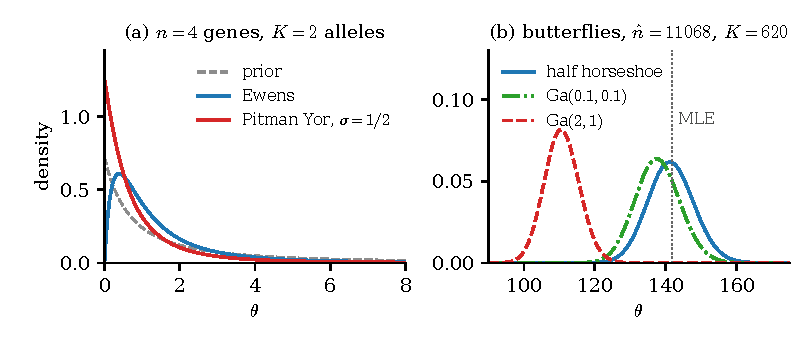
\includegraphics[width=\textwidth]{figures/rc_ewens.pdf}
\caption{(a) Four genes carrying two alleles: the half horseshoe prior and the exact posteriors of Examples~\ref{rc:ex:four} and \ref{rc:ex:py}. (b) Corbet's butterflies, $K=620$ species at $n=\hat n=11068$: posteriors for $\theta$ under three priors, with the maximum likelihood value dotted (Example~\ref{rc:ex:butterflies}).}\label{rc:fig:ewens}
\end{figure}

\section{Numerical Verification and a Simulation Study}\label{rc:sec:numerics}
\sectionmark{Numerical Verification}

\subsection{Verification of the closed forms}

The residue computations of this section use working precision $\lceil N/2\rceil+15$ digits, the rule of remedy (ii) after Proposition~\ref{rc:prop:cond}, and are validated against adaptive quadrature of the unnormalized kernel. Table~\ref{rc:tab:verify} reports the checks; agreement is to every digit shown.

The strip of Theorem~\ref{rc:thm:mellin} is sharp in the numerics as well as in Lemma~\ref{rc:lem:vanish}. For $\rcPPH(2,0.7,6,1,0)$ the left edge is $-1$, since $[\alpha]^2$ vanishes only to first order at the origin; evaluating \eqref{rc:eq:mellin} at $s=-1.7$ returns $-0.0214$, a negative value for a positive integrand, correctly signalling that the identity has been used outside its domain. For $\rcPPH(1,1,5,2,1)$ the left edge is $-2$ and $s=-1.7$ is legitimate, as the table confirms. This is a useful practical warning: the formula does not announce its own failure by blowing up.

\begin{table}[htbp]
\centering\footnotesize
\setlength{\tabcolsep}{3pt}
\begin{tabular}{@{}>{\raggedright\arraybackslash}p{2.05in}rr@{}}
\toprule
Result and setting & Closed form & Quadrature\\
\midrule
Thm.~\ref{rc:thm:residue}, double poles, $R=(\alpha+\frac12)\{(\alpha+1)^2(\alpha+2)^2(\alpha+3)\}^{-1}$ & 0.033206270697541 & 0.033206270697541\\
Thm.~\ref{rc:thm:residue}, complex poles, $R=\{(\alpha+1)((\alpha+2)^2+9)\}^{-1}$ & 0.095487677098166 & 0.095487677098166\\
Thm.~\ref{rc:thm:residue}, Ewens, $n=20$, $k=5$, $\rcPH(0,1,2,1)$ & $1.5311352489\times10^{-19}$ & $1.5311352489\times10^{-19}$\\
Thm.~\ref{rc:thm:mellin}, $s=0.4$, $\rcPH(0,1.1,5,2)$ & 0.00891856126471 & 0.00891856126471\\
Thm.~\ref{rc:thm:mellin}, $s=2.3$, $\rcPH(0,1.1,5,2)$ & 0.000877909609669 & 0.000877909609669\\
Thm.~\ref{rc:thm:mellin}, $s=-0.5$, $\rcPPH(2,0.7,6,1,0)$ & 0.00442197021726 & 0.00442197021726\\
Thm.~\ref{rc:thm:mellin}, $s=-1.7$, $\rcPPH(1,1,5,2,1)$ & 0.0166781629184 & 0.0166781629184\\
Thm.~\ref{rc:thm:tilt}, $z=0.30$, $\rcPH(1,1,4,3)$ & 0.00140806861934 & 0.00140806861934\\
Thm.~\ref{rc:thm:tilt}, improper part, $R=\alpha^2/(\alpha+1.3)$, $z=0.45$ & 0.92288110392933 & 0.92288110392933\\
\bottomrule
\end{tabular}
\caption{Closed forms against adaptive quadrature at thirty digits of working precision.}\label{rc:tab:verify}
\end{table}

\subsection{Does the heavy tail matter? A simulation study}

Corollary~\ref{rc:cor:tail} says the half horseshoe has no moments; Section~\ref{rc:sec:ewens} says the Ewens likelihood carries only $\log n$ worth of information. Together they predict that a light tailed prior will fail to reach a large true concentration and that its credible intervals will undercover. We test this. For $\theta\in\{0.5,2,10\}$ and $n\in\{100,1000\}$ we draw the block count $k$ by the Feller coupling and compute the exact posterior of $\theta$ under three priors: the half horseshoe $\rcPH(0,1,2,1)$, a $\rcGa(2,1)$ prior of the kind used by \citet{rc:escobar1995}, and the diffuse $\rcGa(0.1,0.1)$. Table~\ref{rc:tab:sim} reports root mean squared error of the posterior mean, coverage of the equal tailed $95\%$ interval, and mean interval width over 200 replicates.

\begin{table}[htbp]
\centering\footnotesize
\setlength{\tabcolsep}{2.4pt}
\begin{tabular}{@{}rrrrrrrrrrr@{}}
\toprule
 & & \multicolumn{3}{c}{$\rcPH(0,1,2,1)$} & \multicolumn{3}{c}{$\rcGa(2,1)$} & \multicolumn{3}{c}{$\rcGa(0.1,0.1)$}\\
\cmidrule(lr){3-5}\cmidrule(lr){6-8}\cmidrule(l){9-11}
$\theta$ & $n$ & RMSE & cov & width & RMSE & cov & width & RMSE & cov & width\\
\midrule
0.5 & 100 & 0.359 & 0.97 & 1.44 & 0.455 & 0.94 & 1.62 & 0.362 & 0.91 & 1.36\\
0.5 & 1000 & 0.274 & 0.93 & 1.11 & 0.335 & 0.94 & 1.22 & 0.278 & 0.93 & 1.07\\
2.0 & 100 & 0.817 & 0.94 & 3.14 & \emph{0.641} & 0.97 & 2.80 & 0.849 & 0.93 & 3.20\\
2.0 & 1000 & 0.538 & 0.96 & 2.40 & \emph{0.474} & 0.98 & 2.25 & 0.553 & 0.96 & 2.43\\
10.0 & 100 & 2.585 & 0.94 & 10.15 & 3.196 & \emph{0.61} & 6.26 & 2.434 & 0.94 & 9.77\\
10.0 & 1000 & 1.548 & 0.94 & 6.41 & 2.054 & \emph{0.78} & 5.14 & 1.520 & 0.94 & 6.32\\
\bottomrule
\end{tabular}
\caption{Posterior for the Dirichlet process concentration from the block count, 200 replicates. Italics mark the two effects discussed in the text.}\label{rc:tab:sim}
\end{table}

Three readings, and we report the unfavourable one too. When the truth sits at the prior mean, $\theta=2$, the correctly centred $\rcGa(2,1)$ wins on RMSE by twelve to twenty two per cent, as it should; there is no free lunch, and a heavy tail costs efficiency at the centre. When the truth is large, $\theta=10$, the $\rcGa(2,1)$ posterior cannot follow, and its coverage collapses to 0.61 at $n=100$ and 0.78 at $n=1000$, with intervals that are both too narrow and misplaced. The half horseshoe holds nominal coverage throughout with uniformly lower RMSE than $\rcGa(2,1)$ in that regime. Note also that the diffuse $\rcGa(0.1,0.1)$ is competitive with the half horseshoe everywhere and slightly better at $\theta=10$: the practical gain over a well chosen diffuse Gamma is small, and the case for the Pochhammer prior rests on conjugacy and closed forms rather than on a large risk improvement. What the comparison does establish is that the failure mode of a light tailed default is real and is exactly the one Corollary~\ref{rc:cor:tail} predicts.

\subsection{Conditioning and tails}

Figure~\ref{rc:fig:tails} reports the two remaining experiments. Left, $\log_{10}\kappa_n$ over $n\in\{10,\dots,160\}$ with fit $0.502n-2.30$; at double precision the formula is exhausted by $n\approx36$, a property of the representation and not of the posterior. Right, the marginal $p(n)$ against \eqref{rc:eq:zipf} for $a\in\{1,2\}$; the ratio $p(n)n^{1+a}(\log n)^2/K$ is 1.045 at $n=10^3$ and 0.977 at $n=10^6$ for $a=1$, consistent with the predicted $O(1/\log n)$ correction.

\section{Application: Two Regimes of Overdispersion}\label{rc:sec:app}

Corollary~\ref{rc:cor:tail} says the half horseshoe has no moments, and the simulation study of Section~\ref{rc:sec:numerics} (Table~\ref{rc:tab:sim}) showed that a light tailed Gamma prior fails when the true concentration is large; Example~\ref{rc:ex:butterflies} showed the same failure on the butterflies. This section tests the claim on a second kind of real data, counts with covariates. Two data sets from \citet{rc:venables2002} carry the same model and differ only in regime.
\begin{itemize}
\item \texttt{quine}: days of absence from school for $K=146$ children in New South Wales, with covariates for ethnicity, sex, age band and learner status. Mean 16.5, variance 262, maximum likelihood dispersion $\hat\alpha=1.27$. Strong overdispersion.
\item \texttt{Insurance}: third party motor claims in 64 policy cells, with covariates for district, engine capacity and driver age, and the log number of holders as offset. Mean 49.2, variance 4985. Close to Poisson: the profile likelihood of $\alpha$ increases all the way to its Poisson limit, so the maximum likelihood dispersion is $\hat\alpha=\infty$, and $\alpha$ is bounded below by the data but not above.
\end{itemize}

The model is Negative Binomial regression as in Section~\ref{rc:sec:nb}, $n_i\sim\rcNB(\alpha,\pi_i)$ with $\psi_i=o_i+\bm x_i^\top\bm\beta$, and $\bm\beta\sim N(0,100I)$. We compare three priors on $\alpha$: the half horseshoe $\rcPH(0,1,2,1)$, the diffuse $\rcGa(0.01,0.01)$ and the light tailed $\rcGa(2,1)$. Posterior summaries for \texttt{quine} use $10^5$ retained draws of Algorithm 2. Algorithm 2 does not mix on \texttt{Insurance} (Section~\ref{rc:sec:nblimit}), so there the summaries use $10^5$ draws, four chains of $2.5\times10^4$, from a blocked Metropolis Hastings sampler for the same model: a random walk step on $\log\alpha$ in which $\bm\beta$ is redrawn from its Laplace approximation given the proposed $\alpha$ and the pair is accepted or rejected together, alternated with an independence refresh of $\bm\beta$.

\subsection{Where the prior does not matter}

On \texttt{quine} the three priors are indistinguishable. Panel (a) of Figure~\ref{rc:fig:nbreg} overlays the three posteriors of $\alpha$; the posterior medians are 1.21, 1.21 and 1.22 with essentially identical intervals, and predictive coverage is nominal for all three. This is the expected outcome and we report it as such. With $\sum_in_i=2403$ the likelihood is sharply informative about $\alpha$ near its mode, and no reasonable prior can move it. In this regime the contribution of the present chapter is exactness and conjugacy, not accuracy: Algorithm 2 runs with every block a standard draw and mixes about as well as a tuned random walk Metropolis step for $\alpha$ in the same sampler, at about the same cost per iteration: in four runs of $2\times10^4$ draws each, the effective sample size for $\alpha$ is 520 to 890 for Algorithm 2 against 700 to 810 for random walk Metropolis. What it saves is the tuning, not the time.

\subsection{Where it does}

On \texttt{Insurance} the picture separates, and in the direction Corollary~\ref{rc:cor:tail} predicts. Panel (b) plots the three posteriors on a logarithmic scale. The $\rcGa(2,1)$ posterior sits at a median of 13.1 with a $95\%$ interval $(8.2,20.0)$, in a region the likelihood has all but ruled out: at $\alpha=20$ the profile log likelihood lies 17.7 units below its Poisson limit. Its light tail simply cannot reach the region the data prefer, and because a small $\alpha$ means a large variance function $\mu+\mu^2/\alpha$, the error propagates straight into prediction: the $90\%$ posterior predictive bands, shown in panel (c), have mean width 55.3 against 24.8 for the half horseshoe, with empirical coverage 1.000 rather than the nominal 0.90. The intervals are not merely wrong, they are more than twice as wide as they should be.

The half horseshoe reaches the near Poisson region the likelihood supports, with median 353 and interval $(66,7.4\times10^3)$. That interval is very wide, and deliberately so. Near Poisson data bound $\alpha$ from below but carry almost no information about how large it is, so an honest posterior must be diffuse to the right, and the heavy tail of Corollary~\ref{rc:cor:tail} is what permits it. The episode also shows what Corollary~\ref{rc:cor:tail} means in practice. The prior has no moments, and the posterior mean of $\alpha$ under the half horseshoe, about $2.1\times10^3$ by quadrature, is finite only because the $N(0,100)$ prior on the intercept of $\psi$ penalizes very large $\alpha$; it is six times the median, it is carried by the far right tail, and the average of the $10^5$ draws, 1664, still falls short of it. Under the mean parameterization of Section~\ref{rc:sec:nblimit}, where the likelihood in $\alpha$ tends to a positive constant, the posterior has no mean at all. Posterior medians, not means, are the right summary for this family, and we use them throughout Table~\ref{rc:tab:nbreg}.

\begin{table}[htbp]
\centering\small
\setlength{\tabcolsep}{3.5pt}
\begin{tabular}{@{}llrrrrr@{}}
\toprule
 & & \multicolumn{3}{c}{posterior for $\alpha$} & \multicolumn{2}{c}{$90\%$ predictive}\\
\cmidrule(lr){3-5}\cmidrule(l){6-7}
Data & Prior on $\alpha$ & median & $2.5\%$ & $97.5\%$ & coverage & width\\
\midrule
\texttt{quine} & $\rcPH(0,1,2,1)$ & 1.21 & 0.94 & 1.54 & 0.932 & 49.8\\
$\hat\alpha=1.27$ & $\rcGa(0.01,0.01)$ & 1.21 & 0.94 & 1.54 & 0.938 & 49.8\\
 & $\rcGa(2,1)$ & 1.22 & 0.95 & 1.56 & 0.932 & 49.4\\
\midrule
\texttt{Insurance} & $\rcPH(0,1,2,1)$ & 353.3 & 65.5 & 7433.5 & 0.953 & 24.8\\
$\hat\alpha=\infty$ & $\rcGa(0.01,0.01)$ & 159.8 & 55.2 & 449.2 & 0.953 & 27.0\\
 & $\rcGa(2,1)$ & \emph{13.1} & \emph{8.2} & \emph{20.0} & \emph{1.000} & \emph{55.3}\\
\bottomrule
\end{tabular}
\caption{Negative Binomial regression under three priors on the dispersion. On \texttt{Insurance} the likelihood has no finite maximum ($\hat\alpha=\infty$, the Poisson limit). Italics mark the failure: the $\rcGa(2,1)$ interval lies where the profile log likelihood is at least 17.7 units below its supremum, and its predictive bands are more than twice too wide and overcover.}\label{rc:tab:nbreg}
\end{table}

\subsection{A limitation of Algorithm 2}\label{rc:sec:nblimit}

The second data set also exposes a genuine weakness of our own sampler, which we report rather than tune away. On \texttt{Insurance}, Algorithm 2 yields an effective sample size between 4 and 10 from $2\times10^4$ draws of $\alpha$, in four runs started at $\alpha=20$, 50, 200 and 1000. Panel (d) shows why: the chain drifts rather than mixes.

The cause is not the Chinese restaurant table block and not the exponential scale, since replacing the $\alpha$ draw by a slice sampler on the same conditional changes nothing, giving effective sample sizes between 4 and 16 in the same four runs. The cause is the parameterization. Algorithm 2 is exact precisely because it works with $(\alpha,\psi)$, in which the mean is $\alpha e^{\psi_i}$; when $\alpha$ is large the data identify the product far better than either factor, and $\alpha$ and the intercept lie along a ridge. Any update of $\alpha$ that conditions on $\bm\beta$ must crawl along it.

One remedy is to work with the mean, $\mu_i=e^{\eta_i}$ with $\eta_i=o_i+\bm x_i^\top\bm\beta$, and $\pi_i=\alpha/(\alpha+\mu_i)$, which breaks the ridge and raises the effective sample size to between 13256 and 17526 from $2\times10^4$ draws, a gain of three orders of magnitude at about the same cost per iteration. As run, with $\bm\beta\sim N(0,100I)$ placed on the coefficients of $\eta_i$, this is not a reparameterization of the model stated above but a change of prior: in the coordinates of $\eta$ the intercept prior moves from $N(\log\alpha,100)$ to $N(0,100)$. The change matters only where the likelihood is flat, in the right tail of $\alpha$: under the half horseshoe the posterior median is 395 and the $97.5\%$ point $1.13\times10^4$, against 353 and $7.4\times10^3$ for the stated model. Table~\ref{rc:tab:nbreg} therefore keeps the stated model and breaks the ridge differently, by moving $\alpha$ and $\bm\beta$ together in the blocked sampler described above, which gives effective sample sizes of 8903, 22253 and 14893 for $\log\alpha$ from $10^5$ draws under the three priors. The cost of either remedy is the conjugacy. The blocked sampler replaces the exact draw of $\alpha$ by a joint Metropolis Hastings step, and in the mean parameterization, with $\mu$ fixed, the factor $\pi_i^\alpha$ is no longer of the form $z^\alpha$, so the tilted Pochhammer draw of Theorem~\ref{rc:thm:tilt} is unavailable and $\alpha$ must be slice sampled from its conditional, which is stable in logarithms even though its normalizer is not. The honest summary is that conjugacy and good geometry pull in opposite directions here, that Algorithm 2 is the right choice in the moderate dispersion regime that motivates most count models, and that a sampler which moves $\alpha$ and $\bm\beta$ together should be preferred when $\alpha$ is large.

\begin{figure}[htbp]
\centering
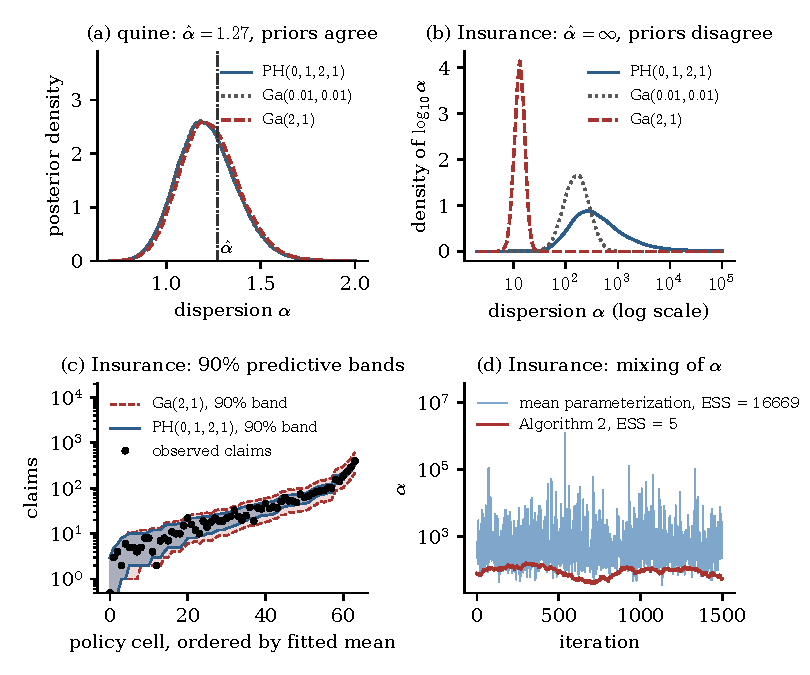
\includegraphics[width=\textwidth]{figures/rc_nbreg.pdf}
\caption{Negative Binomial regression on two data sets. (a) On \texttt{quine} the three priors on the dispersion give the same posterior; the dash dotted line is the maximum likelihood value $\hat\alpha=1.27$. (b) On \texttt{Insurance} they do not: the $\rcGa(2,1)$ posterior sits far below the near Poisson values the likelihood supports, while the half horseshoe reaches them with an honestly diffuse right tail. The likelihood has no finite maximum here, so no $\hat\alpha$ is marked in (b). (c) The consequence for prediction: the $\rcGa(2,1)$ bands are more than twice as wide. (d) Mixing of the dispersion block on \texttt{Insurance}, first 1500 retained draws from a start at $\alpha=20$, with the effective sample size over all $2\times10^4$ draws in the legend; the $(\alpha,\psi)$ ridge that makes Algorithm 2 conjugate is what stalls it. Panels (b) and (c) show the model and sampler of Table~\ref{rc:tab:nbreg}; the mean parameterization trace in (d) comes from the run of Section~\ref{rc:sec:nblimit}, whose prior on the intercept differs.}\label{rc:fig:nbreg}
\end{figure}

\section{Discussion}\label{rc:sec:discussion}

The Pochhammer family is best understood not as a device for Dirichlet Multinomial models but as the conjugate family for the rational likelihoods of applied probability. Posed that way, the tools are partial fractions and the Mellin transform, and the reach is delimited by one criterion, Proposition~\ref{rc:prop:boundary}. Damsleth's class sits just outside it, and we have given the exact repairs available inside.

For population genetics the conclusions are concrete. The scaled mutation rate $\theta$ of the infinitely many alleles model, and its Pitman Yor generalization for fixed discount, admit exact conjugate inference from the allele count alone; the posterior, its moments and the probability that the next gene sampled carries a new allele are finite combinations of logarithms, as Examples~\ref{rc:ex:four} to \ref{rc:ex:py} show by hand. Because the information about $\theta$ grows only like $\log n$, the prior matters at every sample size, and Example~\ref{rc:ex:butterflies} shows that a light tailed Gamma prior of the kind used in the clustering literature can move the answer by almost five standard errors in a sample of 620 species and about eleven thousand individuals. The half horseshoe does not, and Example~\ref{rc:ex:ewhh} shows that it costs nothing in sampling convenience.

Four directions remain. Proposition~\ref{rc:prop:cond}(i) solves one case of the conditioning problem exactly and (ii) leaves the general one open; the natural conjecture is $\log\kappa_n\sim n\,\vartheta(k/n)$ for a rate function $\vartheta$ determined by the pole configuration, obtainable from the same Laplace analysis that yields the leading cancellation. A stable barycentric form of the partial fraction expansion may also exist, by analogy with barycentric rational interpolation. The Mellin representation \eqref{rc:eq:mellin} invites a Mellin Barnes treatment, giving asymptotic expansions of posterior moments in $N$ by shifting contours across poles, and connects the family to generalized Gamma convolutions and Thorin measures; Theorem~\ref{rc:thm:cm} makes that connection concrete, since the mixing law in \eqref{rc:eq:latent} is the size debiased law of a sum of independent exponentials, and whether it lies in the Thorin class is a well posed question we leave open. The regression extension in which each concentration parameter $\alpha_k$ depends on covariates through a log linear link, listed as future work in \citet{rc:wang2024}, is now available through Theorem~\ref{rc:thm:tilt}, since a log linear link contributes exactly a factor $z^\alpha$. Finally, Theorem~\ref{rc:thm:zipf} and Proposition~\ref{rc:prop:boundaryzipf} suggest using the hierarchy as a generative model for heavy tailed counts in its own right, with the Zipf exponent elicited as a hyperparameter and the logarithmic correction supplying a testable refinement of the pure power law.

\section{Exercises}\label{rc:sec:exercises}

\begin{enumerate}[label=\arabic*.,leftmargin=*,itemsep=4pt]
\item Prove the coefficient formula \eqref{rc:eq:pfconv}, and deduce directly that $\sum_i\gamma_i=0$ for $\rcPH(0,a,b,c)$ with $b\ge2$.\\
\emph{Hint.} With $m=d=0$, $\gamma_i=(-1)^{i-1}\binom{b-1}{i-1}/(b-1)!$; use $\sum_j(-1)^j\binom{b-1}{j}=0$.

\item For the half horseshoe $\rcPH(0,1,2,1)$ show that $\E(\alpha^{1/2})=\pi(\sqrt2-1)/\log2=1.8774$ and $\E(\alpha^{-1/2})=\pi(1-2^{-1/2})/\log2=1.3275$, and that $\E(\alpha^{-1})=\E(\alpha)=\infty$.\\
\emph{Hint.} Theorem~\ref{rc:thm:mellin} at $s=\frac32$ and $s=\frac12$, or, for $\E(\alpha^{-1/2})$ alone, directly from $\int_0^\infty\alpha^{s-1}(\alpha+r)^{-1}\dd\alpha=\pi r^{s-1}/\sin(\pi s)$, valid for $0<s<1$.

\item Repeat Example~\ref{rc:ex:four} for four genes carrying three alleles. Show that $C=\frac52-\frac94\log3$, that the posterior mean is $5.0865$, and that the posterior has no variance.\\
\emph{Hint.} The kernel is $\theta^2/\{(\theta+1)^2(\theta+2)^2(\theta+3)\}$, whose integral was already computed in Example~\ref{rc:ex:four}; for the mean use the integral of $\theta^2R$ there.

\item Using the Feller coupling, derive the Fisher information $I_n(\theta)$ of Section~\ref{rc:sec:ewens}, and show that $I_n(\theta)\theta/\log n\to1$.\\
\emph{Hint.} A Bernoulli variable with success probability $p(\theta)$ carries information $p'^2/\{p(1-p)\}$; compare the sum with $\int_1^n\dd x/(\theta+x)$.

\item Show that the Hoppe urn assigns probability $\theta^k\prod_j(n_j-1)!/[\theta]^n$ to every sequence with allele sizes $n_1,\dots,n_k$, and deduce that $K_n$ is sufficient for $\theta$ given the whole sequence.\\
\emph{Hint.} Factorization theorem; the remaining factor does not involve $\theta$.

\item Verify the identity $\theta^k/[\theta]^n=\theta^{k-1}(\theta+n)B(\theta+1,n)/\Gamma(n)$ and derive the mixture weight $w/(1-w)=k/(n\lambda')$ in Example~\ref{rc:ex:ewhh}.\\
\emph{Hint.} Write $B(\theta+1,n)=\int_0^1\eta^\theta(1-\eta)^{n-1}\dd\eta$, then integrate $\theta^{k-1}(\theta+n)e^{-\lambda'\theta}$ term by term.

\item Use Legendre's duplication formula to show that $\Gamma(2\alpha)/\Gamma(\alpha)^2=2^{2\alpha-1}\Gamma(\alpha+\frac12)/\{\sqrt\pi\,\Gamma(\alpha)\}$, and explain via Proposition~\ref{rc:prop:boundary} why no exponential tilt makes the Damsleth marginal with $\nu=2$ rational.\\
\emph{Hint.} The shifts $\frac12$ and $0$ differ by a non integer; $2^{2\alpha}$ is a tilt and cannot cancel infinitely many poles.

\item Compute $\int_0^\infty e^{-\lambda\alpha}\{(\alpha+1)(\alpha+2)\}^{-1}\dd\alpha$ by Theorem~\ref{rc:thm:tilt} and check that it tends to $\log2$ as $\lambda\downarrow0$. At $\lambda=0.01$ it equals $0.65603$.\\
\emph{Hint.} The answer is $e^{\lambda}E_1(\lambda)-e^{2\lambda}E_1(2\lambda)$.

\item Show that for the Pitman Yor model the posterior predictive probability of a new type, $\E\{(\theta+k\sigma)/(\theta+n)\mid\text{data}\}$, is a ratio of two integrals of rational functions, and reproduce the value $0.37867$ of Example~\ref{rc:ex:py}.\\
\emph{Hint.} Multiplying the kernel by $(\theta+k\sigma)/(\theta+n)$ adds one numerator factor and one simple pole.

\item (Computation.) For the kernel of Proposition~\ref{rc:prop:cond} with $k=1$, find the smallest $n$ at which $\kappa_n$ exceeds $10^{16}$, so that double precision returns no correct digits. Then reproduce Table~\ref{rc:tab:digits} and extend it to $n=60$ with 40 digit arithmetic.\\
\emph{Hint.} Use the formula of Proposition~\ref{rc:prop:cond}(i) as a first guess; the answer is $n=51$.

\item (Computation.) Run the sampler of Example~\ref{rc:ex:ewhh} on Corbet's butterflies, with $n=11068$ and $k=620$ as in Example~\ref{rc:ex:butterflies}, and on a sample of your own simulated from the Hoppe urn with $\theta=10$ and $n=200$. Compare the posterior median and $95\%$ interval with those from quadrature of $\theta^{k}[\theta]^{-n}p(\theta)$ in logarithms.\\
\emph{Hint.} Evaluate $\log[\theta]^n$ as $\log\Gamma(\theta+n)-\log\Gamma(\theta)$ to avoid overflow.

\item Show that the posterior of Example~\ref{rc:ex:four} is unimodal, with mode at the unique positive root of $4\theta^3+15\theta^2+9\theta-6=0$, namely $\theta=0.3887$. Compare the mode, median, mean and maximum likelihood estimate, and explain their order.\\
\emph{Hint.} Clear denominators in $1/\theta-2/(\theta+1)-2/(\theta+2)-1/(\theta+3)=0$ and apply Descartes' rule of signs.
\end{enumerate}

\section*{Proofs}\label{rc:app:proofs}\phantomsection

\begin{proof}[Proof of Theorem~\ref{rc:thm:residue}]
Properness gives $R(\alpha)=O(\alpha^{-2})$ at infinity, so the integral converges absolutely; no pole lies on $[0,\infty)$, so the integrand is continuous there. The stated coefficients are the Laurent coefficients at each pole. Multiplying the expansion by $\alpha$ and letting $\alpha\to\infty$ gives $0=\lim\alpha R(\alpha)=\sum_i\gamma_{i1}$. For $j\ge2$ and $r\notin(-\infty,0]$, $\int_0^\infty(\alpha+r)^{-j}\dd\alpha=\{(j-1)r^{j-1}\}^{-1}$. For $j=1$ the individual integrals diverge, so integrate the sum on $[0,T]$: $\sum_i\gamma_{i1}\{\log(T+r_i)-\log r_i\}$. Writing $\log(T+r_i)=\log T+\log(1+r_i/T)$, the first part contributes $\log T\sum_i\gamma_{i1}=0$ and the second vanishes as $T\to\infty$. The branch is principal because the path from $r_i$ to $T+r_i$ stays in $\mathbb{C}\setminus(-\infty,0]$. Nonreal poles occur in conjugate pairs with conjugate coefficients, so the total is real.
\end{proof}

\begin{proof}[Proof of Lemma~\ref{rc:lem:vanish}]
By \eqref{rc:eq:pfconv}, $cR=\sum_i\gamma_i/(\alpha+r_i)$, and the constant factor $c$ changes none of the orders used below. Expanding each simple pole at infinity, $\gamma_i/(\alpha+r_i)=\sum_{k\ge0}\gamma_i(-r_i)^k\alpha^{-k-1}$, so the coefficient of $\alpha^{-k-1}$ in $cR$ is $(-1)^k\sum_i\gamma_ir_i^k$. Since $R=O(\alpha^{m+d-b})$, these vanish for $k+1<b-m-d$, that is $k\le b-m-d-2$. Expanding at the origin, $\gamma_i/(\alpha+r_i)=\sum_{k\ge0}(-1)^k\gamma_ir_i^{-k-1}\alpha^k$, so the coefficient of $\alpha^k$ is $(-1)^k\sum_i\gamma_ir_i^{-k-1}$. Since $[\alpha]^m=\alpha\prod_{s=1}^{m-1}(\alpha+s)$ for $m\ge1$ and equals 1 for $m=0$, we have $R=O(\alpha^{d+\rcone(m\ge1)})$ at the origin, so these vanish for $k\le d+\rcone(m\ge1)-1$, that is $\sum_i\gamma_ir_i^{-k}=0$ for $1\le k\le d+\rcone(m\ge1)$.
\end{proof}

\begin{proof}[Proof of Theorem~\ref{rc:thm:mellin}]
For $0<\operatorname{Re}(s)<1$ and $r>0$, substituting $\alpha=ru$ gives $\int_0^\infty\alpha^{s-1}(\alpha+r)^{-1}\dd\alpha=r^{s-1}B(s,1-s)=\pi r^{s-1}/\sin(\pi s)$. Summing termwise, valid there, gives \eqref{rc:eq:mellin} on that strip. The left side is analytic on $-\{d+\rcone(m\ge1)\}<\operatorname{Re}(s)<b-m-d$ by the growth of $R$ at both endpoints. The right side is meromorphic with possible poles at the integers; at $s=k+1$ for $0\le k\le b-m-d-2$ the pole is cancelled by $\sum_i\gamma_ir_i^k=0$, and at $s=-k+1$ for $1\le k\le d+\rcone(m\ge1)$ by $\sum_i\gamma_ir_i^{-k}=0$, both by Lemma~\ref{rc:lem:vanish}; these are exactly the integers in the strip. Analytic continuation gives the identity throughout. At $s=1$, using $r_i^{s-1}=1+(s-1)\log r_i+\frac12(s-1)^2\log^2r_i+O((s-1)^3)$ and $\pi/\sin(\pi s)=-(s-1)^{-1}+O(s-1)$ together with $\sum_i\gamma_i=0$ gives $\rcM(1)=-c^{-1}\sum_i\gamma_i\log r_i$ and the stated $\rcM'(1)$.
\end{proof}

\begin{proof}[Proof of Corollary~\ref{rc:cor:tail}]
$R(\alpha)\sim c^{-b}\alpha^{m+d-b}$ at infinity, so $\int_x^\infty R\sim c^{-b}x^{m+d-b+1}/(b-m-d-1)$; dividing by $C$ gives the claim. Equivalently, $\rcM$ has a simple pole at the right edge $s=b-m-d$ of the strip, and the Tauberian correspondence for Mellin transforms converts it into regular variation of index $b-m-d-1$.
\end{proof}

\begin{proof}[Proof of Theorem~\ref{rc:thm:tilt}]
The polynomial part contributes
\[
\int_0^\infty e^{-\lambda\alpha}\alpha^k\dd\alpha=k!/\lambda^{k+1}.
\]
For a simple pole, write $c\alpha+a+i-1=c(\alpha+r_i)$ with $r_i=(a+i-1)/c$, and substitute $t=\lambda(\alpha+r_i)$, so that $t$ runs from $\lambda r_i$ to $\infty$ and $e^{-\lambda\alpha}=e^{\lambda r_i}e^{-t}$:
\[
\int_0^\infty\frac{e^{-\lambda\alpha}}{c\alpha+a+i-1}\dd\alpha\;=\;\frac1c\int_0^\infty\frac{e^{-\lambda\alpha}}{\alpha+r_i}\dd\alpha\;=\;\frac1c\,e^{\lambda r_i}\int_{\lambda r_i}^\infty\frac{e^{-t}}{t}\dd t\;=\;\frac1c\,e^{\lambda r_i}E_1(\lambda r_i).
\]
Each of the finitely many terms is absolutely integrable against $e^{-\lambda\alpha}$, so the integral of the sum is the sum of the integrals, and no degree condition is needed because $e^{-\lambda\alpha}$ dominates any polynomial. For the limit, $\Pi\equiv0$ and $e^{\lambda r_i}E_1(\lambda r_i)=-\log\lambda-\log r_i-\rcgE+O(\lambda\log\lambda)$, so the right side of \eqref{rc:eq:tilt} is $-c^{-1}\sum_i\gamma_i\log r_i-c^{-1}(\log\lambda+\rcgE)\sum_i\gamma_i+o(1)$, and $\sum_i\gamma_i=0$ kills the divergent term.
\end{proof}

\begin{proof}[Proof of Proposition~\ref{rc:prop:cond}(ii)]
Write $j=xn$ and $k=\rho n$, so that $\log|\gamma_j|=(k-1)\log j-\log\Gamma(j)-\log\Gamma(n-j)$. Stirling's formula gives
\begin{multline*}
\log|\gamma_{xn}|=\rho n\log(xn)-\{xn\log(xn)-xn\}\\
-\{(1-x)n\log((1-x)n)-(1-x)n\}+O(\log n).
\end{multline*}
The terms carrying $\log n$ collect to $n\log n\{\rho-x-(1-x)\}=(\rho-1)n\log n$, which is free of $x$, and the remainder is $n\Phi(x)$. Hence the maximizer is that of $\Phi$, and $\Phi'(x)=\rho/x-\log x+\log(1-x)=0$ is the stated equation. On $(0,1)$ the left side $\rho/x$ decreases strictly from $+\infty$ to $\rho$ and the right side $\log\{x/(1-x)\}$ increases strictly from $-\infty$ to $+\infty$, so the root is unique and is a maximum.
\end{proof}

\begin{proof}[Proof of Theorem~\ref{rc:thm:zipf}]
Write $u=(1+c)\alpha+a$. Integrating out $\pi$, $p(n\mid\alpha)=[\alpha]^nB(u,b+n)/\{n!\,B(c\alpha+a,b)\}$. As $n\to\infty$, $[\alpha]^n/n!\sim n^{\alpha-1}/\Gamma(\alpha)$ and $B(u,b+n)\sim\Gamma(u)n^{-u}$, uniformly on compact subsets of $[0,\infty)$. Hence $p(n\mid\alpha)\sim\rcK(\alpha)n^{-c\alpha-a-1}$ with $\rcK(\alpha)=\Gamma\{(1+c)\alpha+a\}/\{\Gamma(\alpha)B(c\alpha+a,b)\}$. Since $\Gamma(\alpha)^{-1}=\alpha+O(\alpha^2)$ at the origin, $\rcK(\alpha)=\alpha\Gamma(a)/B(a,b)+O(\alpha^2)$, and $p_\alpha(\alpha)=\varpi\alpha^{\rcone(m\ge1)}+O(\alpha^{1+\rcone(m\ge1)})$ by the same first order vanishing of $[\alpha]^m$. With $L=\log n$,
\[
p(n)\sim n^{-a-1}\int_0^\infty e^{-cL\alpha}\rcK(\alpha)p_\alpha(\alpha)\dd\alpha,
\]
and Watson's lemma applies. With $\iota=1+\rcone(m\ge1)$ we have $\rcK p_\alpha=\varpi\Gamma(a)B(a,b)^{-1}\alpha^\iota+O(\alpha^{\iota+1})$ and $\int_0^\infty\alpha^\iota e^{-cL\alpha}\dd\alpha=\Gamma(1+\iota)/(cL)^{1+\iota}$, which gives \eqref{rc:eq:zipf} with relative error $O(1/L)$.
\end{proof}

\begin{proof}[Proof of Proposition~\ref{rc:prop:cond}(i)]
With $k=1$, $R(\alpha)=\prod_{i=1}^{n-1}(\alpha+i)^{-1}$ and $\gamma_j=\prod_{i\ne j}(i-j)^{-1}=(-1)^{j-1}/\{(j-1)!(n-1-j)!\}$, so $|\gamma_j|=\binom{n-2}{j-1}/(n-2)!$. The central binomial coefficient is the largest, so the maximum is attained at $j-1=\lfloor(n-2)/2\rfloor$ and equals $\binom{n-2}{\lfloor(n-2)/2\rfloor}/(n-2)!\sim2^{n-2}\{2/(\pi n)\}^{1/2}/(n-2)!$ by Stirling. For the normalizer, $R(\alpha)=\Gamma(\alpha+1)/\Gamma(\alpha+n)$. Substitute $\alpha=u/\log n$; since $\Gamma(n)/\Gamma(n+u/\log n)=e^{-u}\{1+O(1/n)\}$ uniformly for $u$ in compacts, and $\Gamma(1+u/\log n)\to1$, dominated convergence together with $\Gamma(1+x)=1+O(x)$ gives
\[
(n-1)!\int_0^\infty R\;=\;\frac{1}{\log n}\int_0^\infty\Gamma\Bigl(1+\frac{u}{\log n}\Bigr)\frac{\Gamma(n)}{\Gamma(n+u/\log n)}\dd u\;=\;\frac{1+O(1/\log n)}{\log n}.
\]
Dividing, $\kappa_n=\binom{n-2}{\lfloor(n-2)/2\rfloor}(n-1)\log n\{1+O(1/\log n)\}$, which is the stated formula. Numerically, $\log_{10}\kappa_n$ equals 3.171, 6.465, 12.733, 25.001 and 49.298 at $n=10,20,40,80,160$, against 3.127, 6.425, 12.698, 24.970 and 49.269 from the asymptotic formula; the gap, between $0.03$ and $0.05$ in the logarithm, is the $O(1/\log n)$ factor.
\end{proof}

\begin{proof}[Proof of Proposition~\ref{rc:prop:boundaryzipf}]
$\rho B(n,\rho+1)=\rho\Gamma(n)\Gamma(\rho+1)/\Gamma(n+\rho+1)\sim\rho\Gamma(\rho+1)n^{-(1+\rho)}$. Integrating against $p_\rho$ and writing $n^{-\rho}=e^{-\rho\log n}$, Watson's lemma with $\rho\Gamma(\rho+1)p_\rho(\rho)=p_\rho(0)\rho+O(\rho^2)$ gives $p(n)\sim p_\rho(0)n^{-1}(\log n)^{-2}$. Summability follows from the integral test.
\end{proof}

\section*{Implementation notes}\label{rc:app:impl}\phantomsection

The evaluation is short. Given poles $r_i$ with multiplicities $\mu_i$ and numerator $P$, form $h_i(\alpha)=P(\alpha)\prod_{l\ne i}(\alpha+r_l)^{-\mu_l}$, analytic at $-r_i$, and set $\gamma_{ij}=h_i^{(\mu_i-j)}(-r_i)/(\mu_i-j)!$; then apply \eqref{rc:eq:residue}, or \eqref{rc:eq:tilt} if a tilt is present. Set working precision to $\lceil N/2\rceil+15$ digits for kernels like those of Section~\ref{rc:sec:numerics}; a kernel with $k/n$ near $0.15$ needs about $0.54N$. Before using the result, check the graded diagnostics of Lemma~\ref{rc:lem:vanish}: the largest $k$ for which $|\sum_i\gamma_ir_i^k|/\max_i|\gamma_ir_i^k|$ is still at the precision floor reports the achieved accuracy, and a failure at $k=0$ means the answer is noise.

\begin{thebibliography}{99}

\bibitem[Bondesson(1992)]{rc:bondesson1992}
Bondesson, L. (1992). \emph{Generalized Gamma Convolutions and Related Classes of Distributions and Densities}. Lecture Notes in Statistics 76, Springer, New York.

\bibitem[Carvalho et~al.(2010)]{rc:carvalho2010}
Carvalho, C.~M., Polson, N.~G., and Scott, J.~G. (2010). The horseshoe estimator for sparse signals. \emph{Biometrika}, 97(2), 465 to 480.

\bibitem[Damsleth(1975)]{rc:damsleth1975}
Damsleth, E. (1975). Conjugate classes for gamma distributions. \emph{Scandinavian Journal of Statistics}, 2(2), 80 to 84.

\bibitem[Datta and Dunson(2016)]{rc:datta2016}
Datta, J. and Dunson, D.~B. (2016). Bayesian inference on quasisparse count data. \emph{Biometrika}, 103(4), 971 to 983.

\bibitem[Escobar and West(1995)]{rc:escobar1995}
Escobar, M.~D. and West, M. (1995). Bayesian density estimation and inference using mixtures. \emph{Journal of the American Statistical Association}, 90(430), 577 to 588.

\bibitem[Ewens(1972)]{rc:ewens1972}
Ewens, W.~J. (1972). The sampling theory of selectively neutral alleles. \emph{Theoretical Population Biology}, 3(1), 87 to 112.

\bibitem[Fisher et~al.(1943)]{rc:fisher1943}
Fisher, R.~A., Corbet, A.~S., and Williams, C.~B. (1943). The relation between the number of species and the number of individuals in a random sample of an animal population. \emph{Journal of Animal Ecology}, 12(1), 42 to 58.

\bibitem[Goldie(1967)]{rc:goldie1967}
Goldie, C.~M. (1967). A class of infinitely divisible random variables. \emph{Mathematical Proceedings of the Cambridge Philosophical Society}, 63(4), 1141 to 1143.

\bibitem[He et~al.(2019)]{rc:he2019}
He, J., Polson, N.~G., and Xu, J. (2019). Data augmentation with P\'olya inverse Gamma. arXiv:1905.12141.

\bibitem[He et~al.(2021)]{rc:he2021}
He, J., Polson, N.~G., and Xu, J. (2021). Bayesian inference for Gamma models. arXiv:2106.01906.

\bibitem[Hoppe(1984)]{rc:hoppe1984}
Hoppe, F.~M. (1984). P\'olya like urns and the Ewens sampling formula. \emph{Journal of Mathematical Biology}, 20(1), 91 to 94.

\bibitem[Miller(2019)]{rc:miller2019}
Miller, J.~W. (2019). Fast and accurate approximation of the full conditional for gamma shape parameters. \emph{Journal of Computational and Graphical Statistics}, 28(2), 476 to 480.

\bibitem[Minka(2000)]{rc:minka2000}
Minka, T.~P. (2000). Estimating a Dirichlet distribution. Technical report.

\bibitem[Pitman(2006)]{rc:pitman2006}
Pitman, J. (2006). \emph{Combinatorial Stochastic Processes}. Lecture Notes in Mathematics 1875, Springer.

\bibitem[Polson and Scott(2011)]{rc:polson2010}
Polson, N.~G. and Scott, J.~G. (2011). Shrink globally, act locally: sparse Bayesian regularization and prediction. \emph{Bayesian Statistics}, 9, 501 to 538.

\bibitem[Polson et~al.(2013)]{rc:polson2013}
Polson, N.~G., Scott, J.~G., and Windle, J. (2013). Bayesian inference for logistic models using P\'olya Gamma latent variables. \emph{Journal of the American Statistical Association}, 108(504), 1339 to 1349.

\bibitem[Simon(1955)]{rc:simon1955}
Simon, H.~A. (1955). On a class of skew distribution functions. \emph{Biometrika}, 42(3/4), 425 to 440.

\bibitem[Steutel(1967)]{rc:steutel1967}
Steutel, F.~W. (1967). Note on the infinite divisibility of exponential mixtures. \emph{Annals of Mathematical Statistics}, 38(4), 1303 to 1305.

\bibitem[van Dyk and Park(2008)]{rc:vandyk2008}
van Dyk, D.~A. and Park, T. (2008). Partially collapsed Gibbs samplers: theory and methods. \emph{Journal of the American Statistical Association}, 103(482), 790 to 796.

\bibitem[Venables and Ripley(2002)]{rc:venables2002}
Venables, W.~N. and Ripley, B.~D. (2002). \emph{Modern Applied Statistics with S}, fourth edition. Springer, New York.

\bibitem[Wang and Polson(2024)]{rc:wang2024}
Wang, Y. and Polson, N.~G. (2024). Pochhammer priors for sparse count models. arXiv:2402.09583.

\bibitem[Zhou and Carin(2015)]{rc:zhou2015}
Zhou, M. and Carin, L. (2015). Negative binomial process count and mixture modeling. \emph{IEEE Transactions on Pattern Analysis and Machine Intelligence}, 37(2), 307 to 320.

\bibitem[Zito et~al.(2026)]{rc:zito2024}
Zito, A., Rigon, T., and Dunson, D.~B. (2026). Bayesian nonparametric modeling of latent partitions via Stirling gamma priors. \emph{Bayesian Analysis}, 21(1), 139 to 166, doi:10.1214/24\nobreakdash-BA1463.

\end{thebibliography}
